% !TEX root = ../PhD Thesis.tex
\chapter{CompBio app server}
\label{chap:app-server}

Since I started building psichomics, I wanted my work to be publicly available as an online web app, providing users the most up-to-date version at their fingerprints, without having to install, update and manage different versions of R, Bioconductor, psichomics and all their dependencies.
%It can take an hour to install psichomics from scratch and the command line may scare the end-users for whom psichomics was created. 
Five years after the first Bioconductor release of psichomics in 2016, that vision finally came true.

\begin{figure}[!b]
  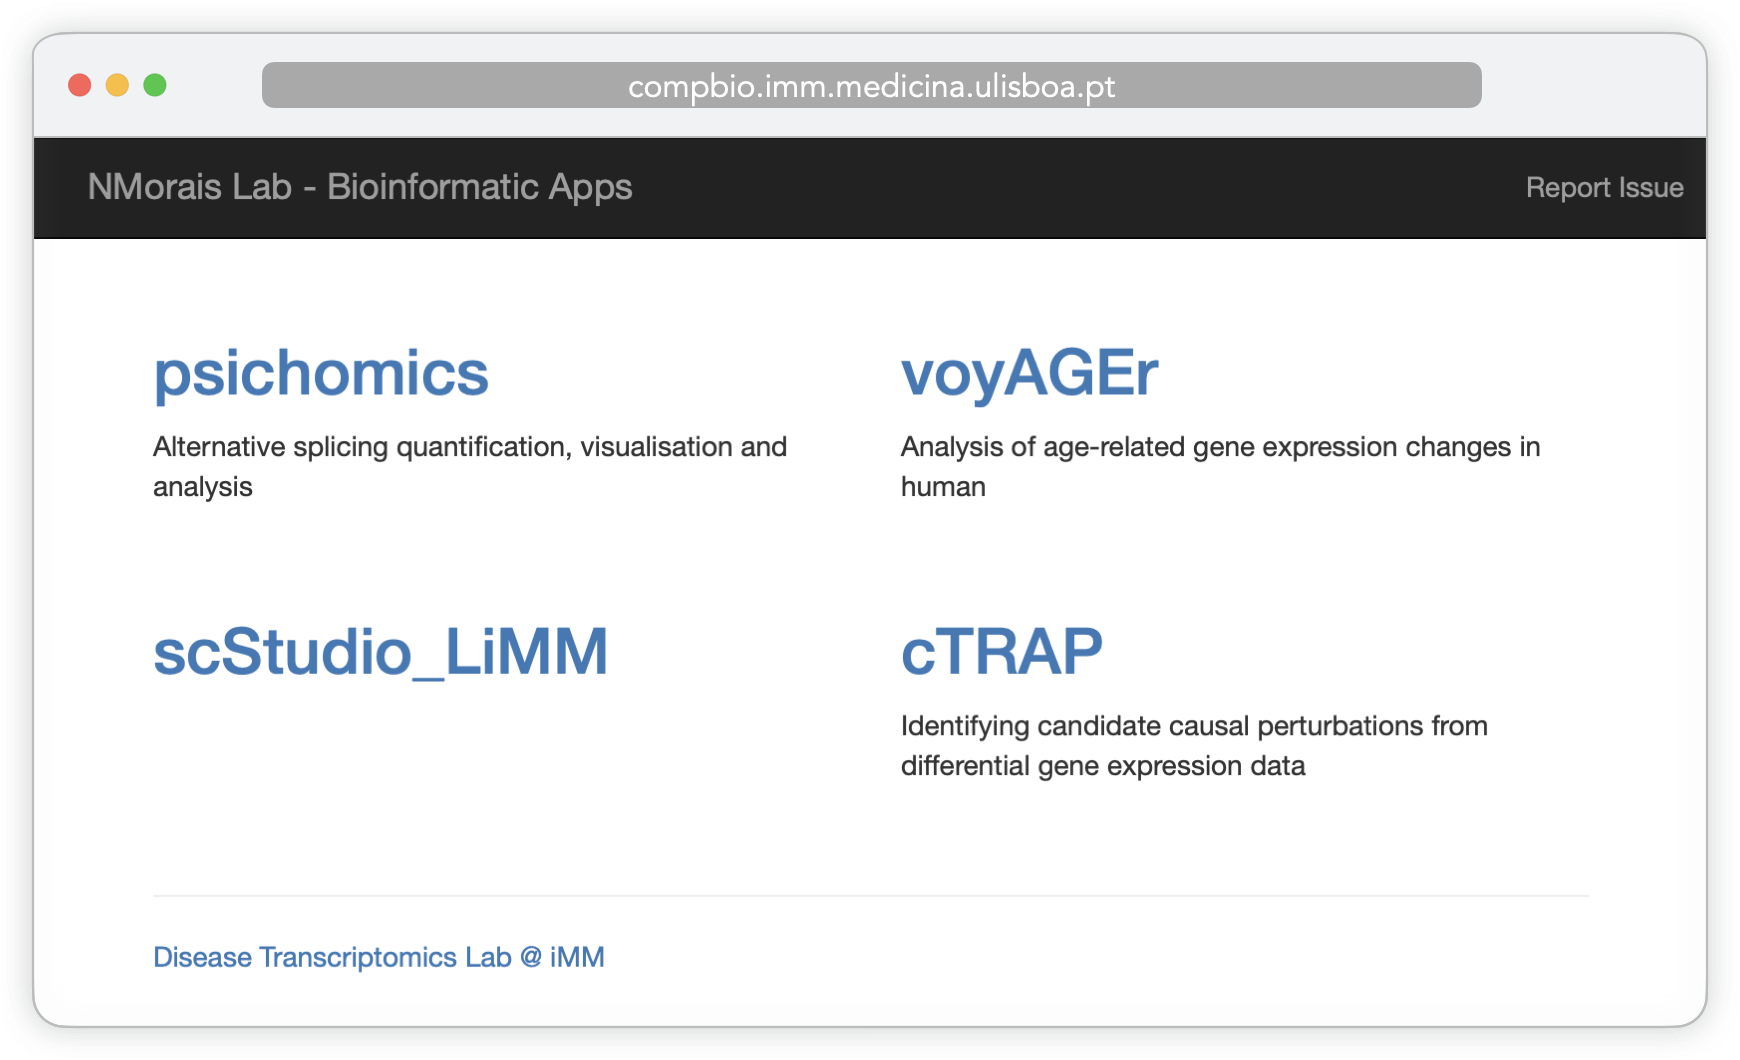
\includegraphics[width=.89\textwidth]{images/app-server/homepage}
  \centering
  \caption[Screenshot of CompBio's homepage]{\textbf{CompBio's homepage screenshot.} List of hosted web apps (11 Nov 2021).}
  \label{fig:homepage}
\end{figure}

One of our lab's ambitious goals is to develop interactive visual tools to assist in exploring biological data, either provided by users or available from big datasets. We want our tools to be used by anyone, no matter their computational background. To turn that dream into reality, I set up the CompBio app server, a Linux virtual machine running in the iMM computing cluster that hosts psichomics, cTRAP and other Shiny apps from my lab colleagues. The server is accessible at \alink{compbio.imm.medicina.ulisboa.pt} (\autoref{fig:homepage}) and its code at \alink{github.com/nuno-agostinho/compbio-app-server}.

% TODO: write specs of the app server? 200GB SSD, 64GB RAM, 16 CPU threads

\section{Background}

Our lab uses the R statistical language to analyse clinical and molecular data from public sources and collaborators. In order to share data insights with our collaborators or even the whole scientific community, we have been increasingly creating exploratory dashboards using the Shiny R package \cite{chang:2021ul}. While developing interactive Shiny web apps, it is natural to wonder: what is the best way to share them?

\subsection{Desktop apps}

Shiny apps are written in R, an interpreted programming language whose source code can run in multiple platforms \cite{r-core-team:2021wf,chang:2021ul}. When run locally, the Shiny app starts running in the device itself (\texttt{localhost}) and is accessible via a web browser. Shiny apps can be part of an R package and be provided in CRAN or Bioconductor (such as in the case of psichomics and cTRAP). Nonetheless, this requires the user to install multiple programs in their computer: R, Shiny, the Shiny app, and all their dependencies. This can take up some time if the user does not have R and many of the required libraries installed. For instance, installing psichomics in a new system can take up to 1 hour. Moreover, it still requires opening an R session to start the visual interface, which may discourage technically-challenged users to try out psichomics.

% Java (\alink{java.com}) is a platform-independent, general-purpose programming language intended to allow the same code to target multiple platforms. It uses an intermediary Java virtual machine (JVM) that translates Jave bytecode to the native platform's language. On the other hand, graphical interfaces in Java can consume more time and memory than native apps, besides having a user interface that is in stark contrast to the graphical interface of other apps.

One way to reduce the number of dependencies installed is by using Docker (\alink{docker.com}), allowing to run isolated Linux virtual environments (containers) that already contain programs and all their dependencies set up. This approach simply requires end-users to install Docker and to download the desired Docker images online. Still, Docker is a program that needs administrator privileges for installation that (1) not all users may have and (2) may not feel comfortable to give to a software they would not otherwise install.

An alternative is Electron (\alink{electronjs.org}), a software framework that allows to develop cross-platform graphical user interface apps using web technologies by combining a web browser rendering engine (Chromium, used in Chrome and other web browsers to convert HTML and CSS code into an interactive web page) and a JavaScript environment. The app itself runs the web app as if it were a usual desktop app. Some open-source projects like electricShine (\alink{github.com/chasemc/electricShine}) and photon (\alink{github.com/COVAIL/photon}) allow to convert Shiny apps to Electron apps, but they are still not fully developed and lack important features (like support for some operative systems). Regardless, compared to native apps, Electron apps are slower, have a significant overhead, take more space and consume more RAM, making Electron less attractive for intensive data-processing apps.

\subsection{Web apps}

Web apps are cross-platform, always up-to-date and can be accessed by any (modern) web browser, making access to such apps easier for end-users \cite{silva:2017wl}. However, a constantly online web server needs to be running and share its computing resources (e.g. amount of RAM, storage and CPU threads) across multiple users. The resources allocated to a web server depend on the resources consumed per app, the number of simultaneous users and the data stored per user. The price of components and their maintenance is specially relevant if anticipating a large number of end-users.

Multiple web app hosting services support Shiny apps or Docker containers of Shiny apps, including Heroku (\alink{heroku.com}) and \alink{shinyapps.io}. Both of these app hosting services offer subscription plans depending on allocated system resources, including a free plan useful to run basic apps: Heroku's free plan offers 2 threads, 512 MB of RAM and 500 MB of storage per app\footnote{According to Heroku (\alink{heroku.com/pricing} and \alink{devcenter.heroku.com/articles/limits}) as of 24 November 2021. Unverified accounts (i.e. not associated with a valid credit card) are limited to 5 apps.}, whereas \alink{shinyapps.io}'s free plan allows for 5 apps with 25 computing hours per month using 1024 MB of RAM and 1 GB of storage per app\footnote{According to official \alink{shinyapps.io} documentation (\alink{docs.rstudio.com/shinyapps.io/applications.html} and \alink{shinyapps.io\#pricing}) as of 24 November 2021.}. Such services take care of deploying the web apps and we can select a different plan to scale up the required resources to run the apps, depending on their usage. They also allow to monitor app resource usage and understand how the apps are being used and if the resources employed are sufficient or not without much effort to the developer.

Besides third-party server hosting, Shiny apps can also be deployed in local web servers. This requires server maintenance and may be harder to scale resources because of higher up-front costs. The following programs allow to locally host Shiny apps:

\begin{itemize}
	\item \textbf{Shiny Server} (\alink{rstudio.com/products/shiny/shiny-server}) is a bare-featured open-source program with only the essential features to host Shiny apps.
	\item \textbf{RStudio Connect} (\alink{rstudio.com/products/connect}) is a paid program\footnote{According to RStudio (\alink{rstudio.com/pricing}), all RStudio commercial products are free for teaching purposes and 50\% discounted for academic research from their regular bundle pricing starting at 22000\$ per year as of 24 November 2021.} with many more features than Shiny Server, including user authentication, Python-based app support and resource usage metrics.
	\item \textbf{ShinyProxy} (\alink{shinyproxy.io}) is an open-source program to host Shiny apps in Docker containers with many of the features found in RStudio Connect, including user authentication, Python-based app support and resource usage metrics.
\end{itemize}

Given that we have sufficient computing resources at our lab's disposal, we decided to build an app server -- a web server dedicated to deploy our web apps. We decided to use ShinyProxy as it has many of the advantages of using the proprietary RStudio Connect for free. Following this choice, we had to think how to properly develop the web server so it is easy to maintain, update and add new apps.

% Nginx as reverse proxy to handle all requests, including SSL certificates for HTTPS
% Nginx as a reverse proxy, serves as an intermediary between the user requests and the server.

In this chapter, I describe CompBio, our app server built with Docker Compose, a program to simultaneously manage multiple interacting Docker containers to allow for R/Shiny and Python app deployment (ShinyProxy) over a reverse proxy (Nginx), background tasks (Celery, Redis and Flower), website analytics (Plausible, PostgreSQL and ClickHouse), resource monitoring (Prometheus and Grafana), and feature testing (RStudio Web, only used to develop features and R scripts). CompBio is currently running in a virtual machine in a Linux computing cluster and hosts Shiny apps from NMorais lab, including the tools previously mentioned in this document: psichomics and cTRAP. CompBio is so named because it powers \textbf{Comp}utational \textbf{Bio}logy apps.

\section{Materials and methods}

CompBio is built using Docker Compose to manage the Docker images of multiple services: ShinyProxy, Nginx, Celery, Redis, Flower, Plausible, PostgreSQL, ClickHouse, Prometheus, Grafana and RStudio Web (\autoref{tab:compbio-services}). 
RStudio Web is only available in the development profile. The services communicate between each other via a single network created by Docker (\autoref{fig:architecture}).

\begin{table}[!h]
\small
\caption[CompBio web services]{\textbf{CompBio services.}}
\label{tab:compbio-services}
\begin{tabularx}{\textwidth}{ l l r l }
\toprule
\parnoteclear
\textbf{Role}                         & \textbf{Service} & \textbf{Port} & \textbf{Docker image}\parnote{Available in Docker Hub, unless stated otherwise.} \\
\toprule
Web app deployment                    & ShinyProxy     & 8080 & \dockerlink{openanalytics/shinyproxy}     \\ \midrule
Reverse proxy                         & Nginx          &  443 & \dockerlink[_]{nginx}     \\ \midrule
\multirow{3}{4cm}{Background tasks} & Celery + cTRAP &      & Based on \dockerlink{nunoagostinho/ctrap}\parnote{Python and Celery are installed on top of cTRAP Docker image, allowing Celery to run cTRAP analyses: see file \link{https://github.com/nuno-agostinho/compbio-app-server/blob/main/celery/Dockerfile}{celery/Dockerfile}.} \\
                                      & Redis          &      & \dockerlink[_]{redis}     \\
                                      & Flower         & 5555 & \dockerlink{mher/flower}     \\ \midrule
\multirow{3}{4cm}{Website analytics
\par(i.e. track visitor metrics)}     & Plausible      & 8000 & \dockerlink{plausible/analytics}     \\
                                      & PostgreSQL     & 5432 & \dockerlink[_]{postgres}     \\
                                      & ClickHouse     &      & \dockerlink{yandex/clickhouse-server}     \\ \midrule
\multirow{4}{4cm}{Resource monitoring} & Prometheus     & 9090 & \dockerlink{prom/prometheus}     \\
                                      & Grafana        & 3000 & \dockerlink{grafana/grafana}     \\
& Nginx monitoring & & \dockerlink{nginx/nginx-prometheus-exporter}     \\
& System monitoring  & & \dockerlink{prom/node-exporter}     \\ \midrule
RStudio (testing) & RStudio Web\parnote{Only available in the development profile.} & 8787 & Based on \dockerlink{rocker/rstudio} \\
\bottomrule
\end{tabularx}
\parnotes
\end{table}

\begin{figure}[!h]
  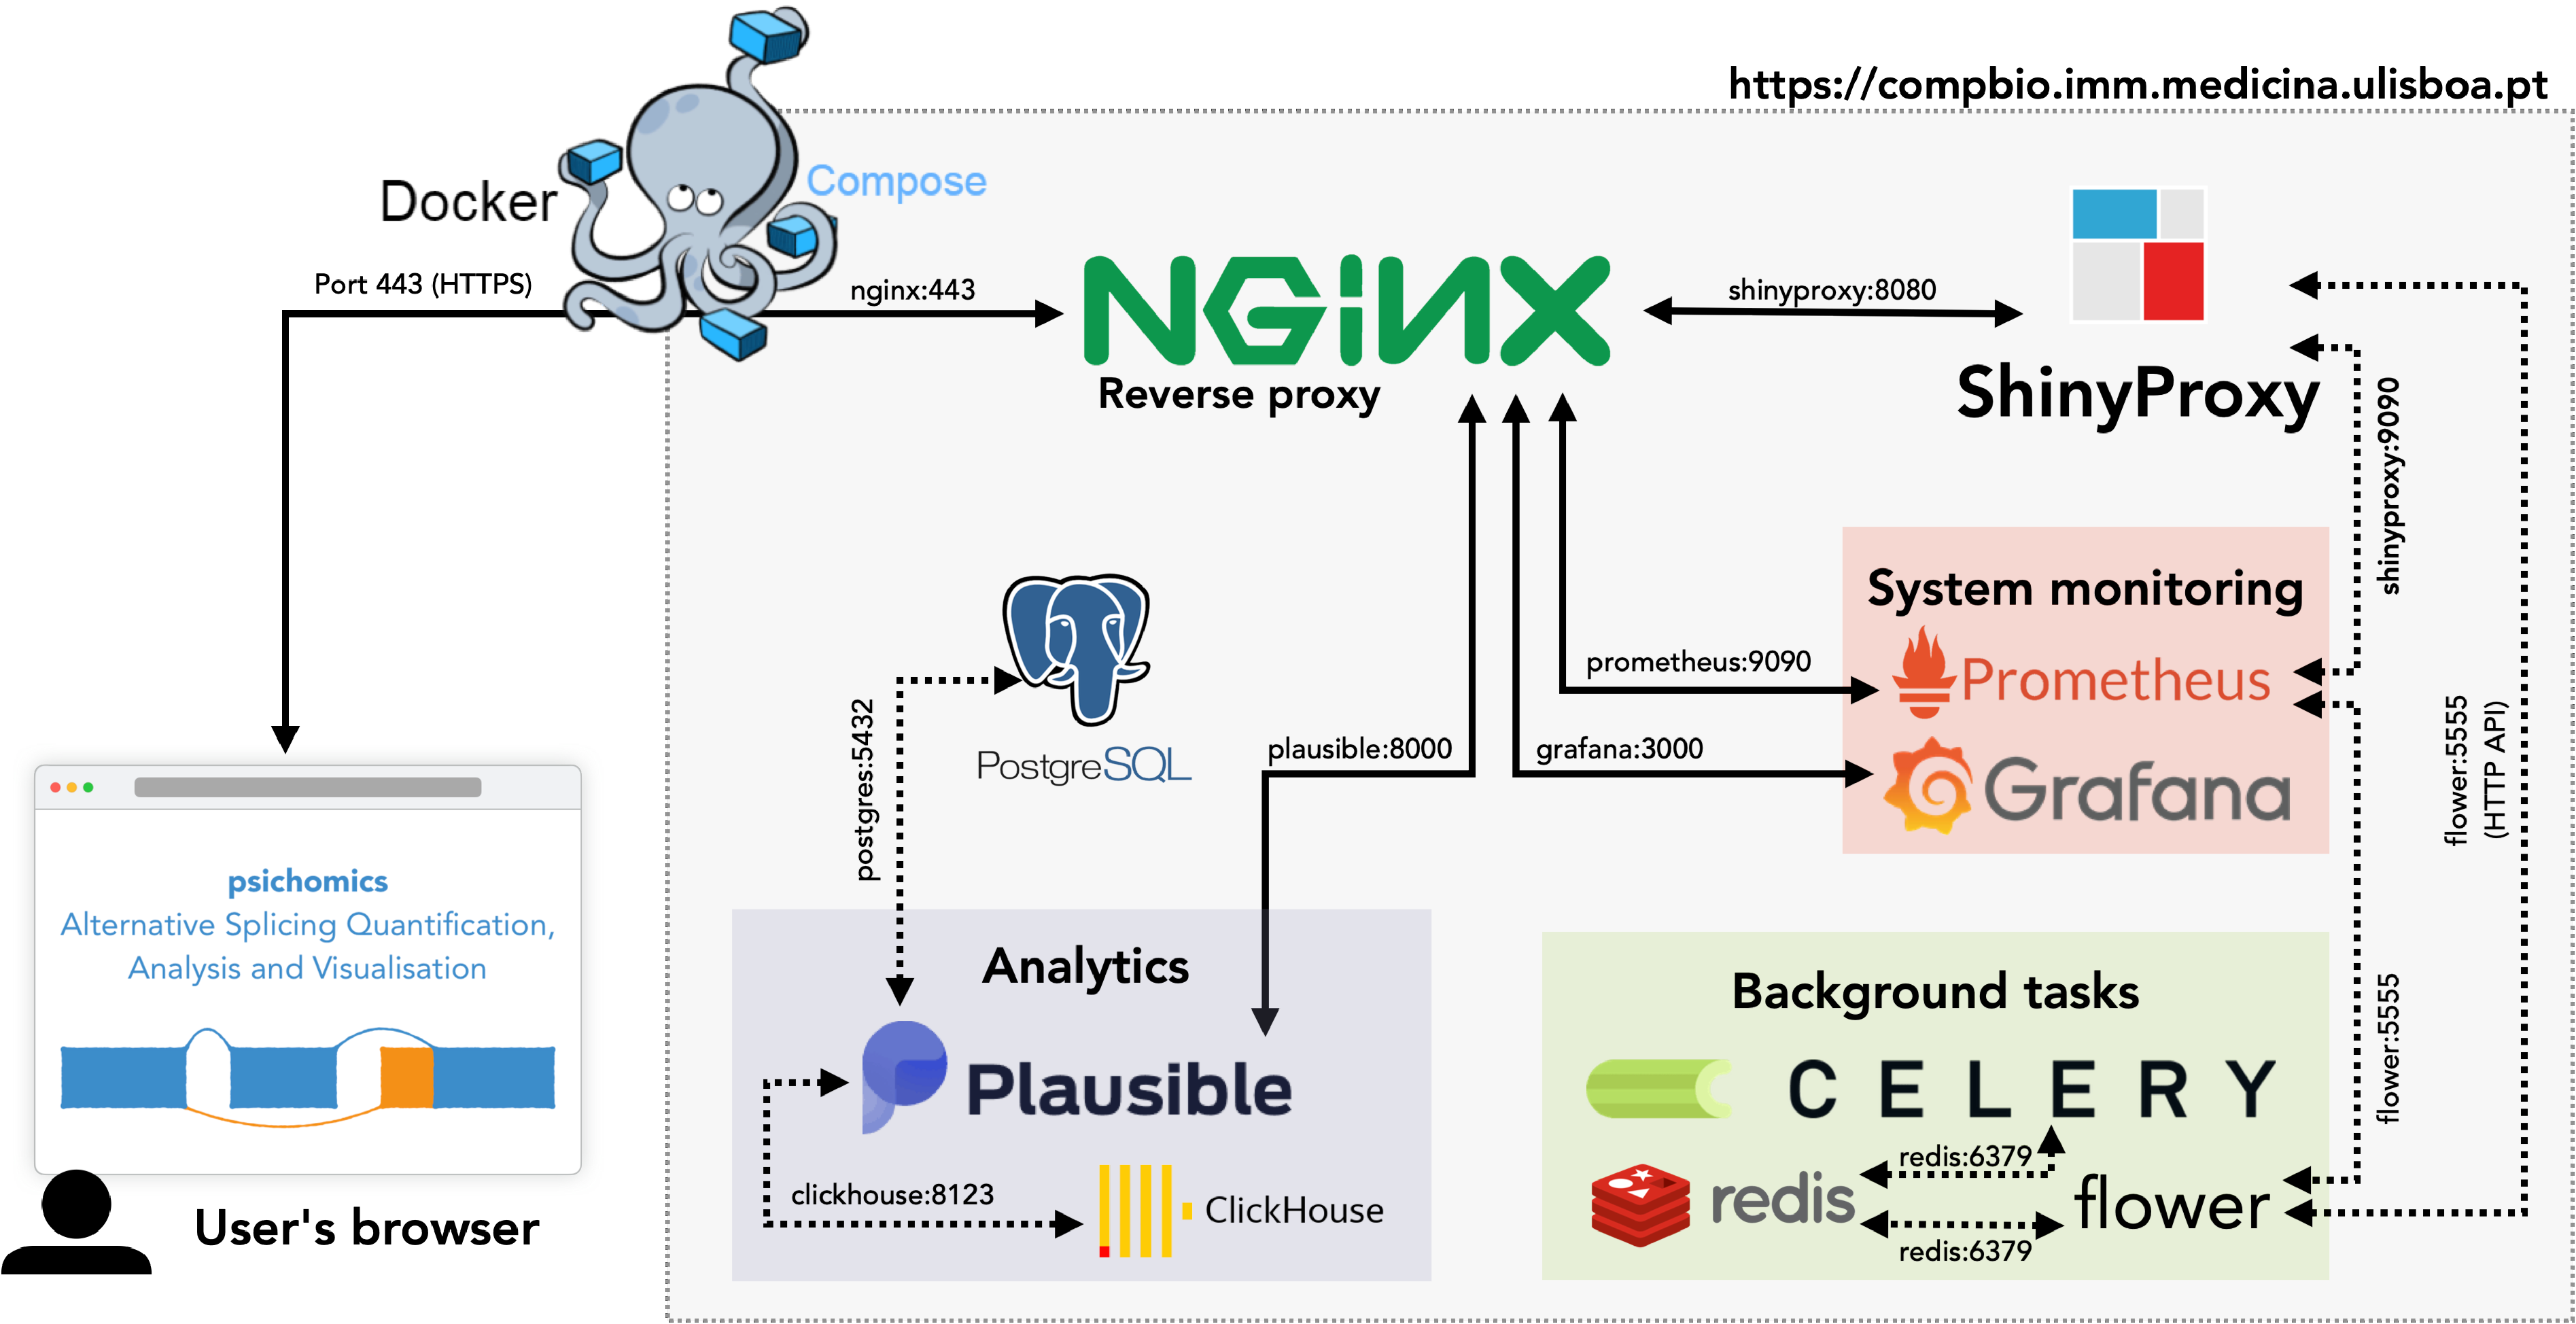
\includegraphics[width=.9\textwidth]{images/app-server/architecture}
  \centering
  \caption[App server architecture]{\textbf{App server architecture is based on Docker Compose.} All services are provided via Docker images and communicate with each other via a Docker-created network using the name of the service and a specific port (e.g. Nginx communicates with ShinyProxy via \texttt{shinyproxy:8080}). The groups  (analytics, system monitoring and background tasks) are strictly conceptual.}
  \label{fig:architecture}
\end{figure}

Services whose ports are listed in \shortref{tab:compbio-services} may be accessed when connected via an ethernet cable at iMM or via the VPN of Universidade de Lisboa by using an internal HTTP (not HTTPS) URL specifying the service port. For instance, opening \link{http://imm-nmorais-p2.fm.ul.pt:8000}{http://imm-nmorais-p2.fm.ul.pt:8000} allows to access the Plausible dashboard\footnote{If the web browser starts redirecting HTTP requests to HTTPS, the website should be accessed in private mode to avoid that behaviour, given that HTTPS disallows specifying ports.}.

\section{Results}

The CompBio app server was developed to be easily maintained and extended, allowing to add new and update existing Shiny apps and other modules. The server also supports running background processes\footnote{More information in \fullref{sec:background-tasks}.}, tracking simple visitor metrics (e.g. Shiny app usage time, number of visitors and user countries) and monitoring system usage. This project is open-source and free (\alink{github.com/nuno-agostinho/compbio-app-server}) and the app server can be publicly accessed at \alink{compbio.imm.medicina.ulisboa.pt}.

The app server makes use of a two-tiered architecture as the user interface is displayed using the user's web browser to render the HTML, CSS and JavaScript code, whereas the application and database layers are all run in the same server. The server itself is a virtual machine running in Lobo (iMM computing cluster) with 16 CPU threads, 64GB RAM and 200GB SSD. By exploiting a powerful infrastructure, the virtual machine can be manually modified to increase or decrease associated computing resources depending on system usage.

The code can be run on Linux\footnote{Although not the scope of this project, CompBio may be compatible with other operating systems.} machines with Docker Compose installed, thus making the setup easily portable and requiring minimal user setup. Docker Compose also confers modularity and maintainability to the project, given that system components are easy to update and replace without affecting other components.

\subsection{Docker Compose}

There are a lot of programs that can go into a web server. Experimenting different programs while managing their manifold dependencies to develop an healthy web server is like an intricate ballet where all finely-coordinated dancers interplay for an astounding performance: a wrong move can affect the whole show. After all, each program/dependency has its own requirements and some may be a distress to (un)install. Moreover, when the server is online, errors may arise due to configuration changes (such as new app updates), requiring a fast rollback to minimise server downtime. A solution is to use self-contained and modular programs, such as Docker containers. But how to coordinate several artists to beautifully perform the Swan Lake?

\begin{figure}[!b]
  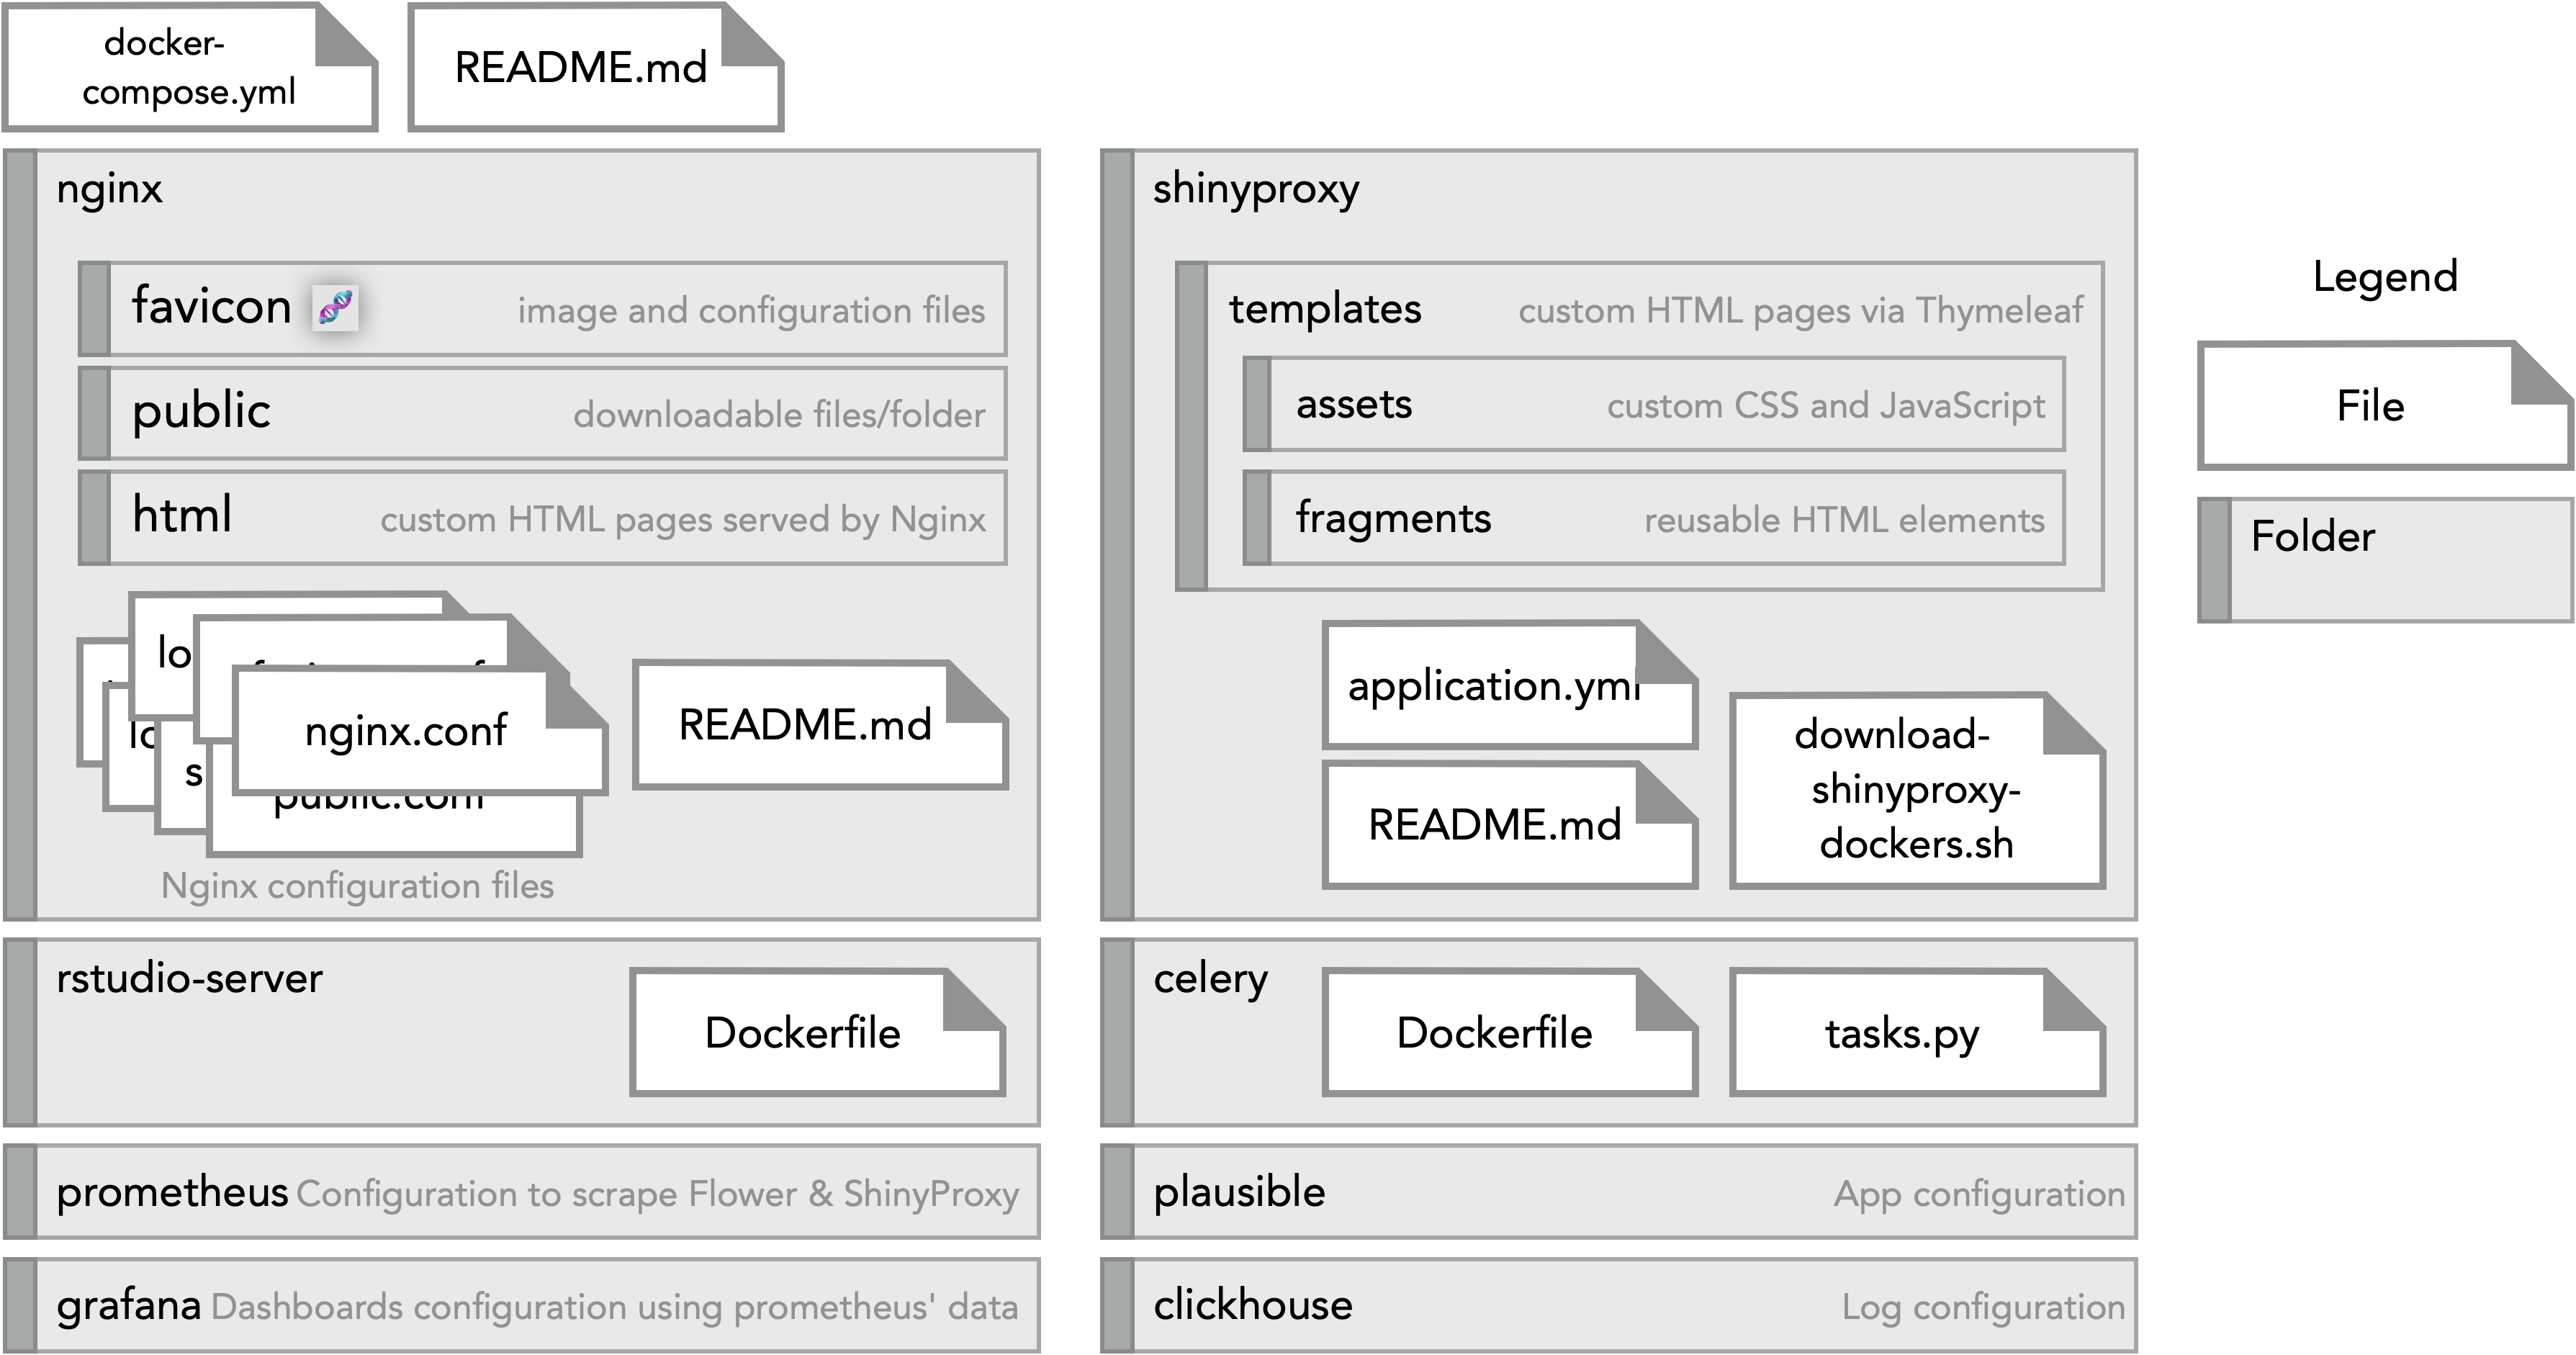
\includegraphics[width=1\textwidth]{images/app-server/file-structure}
  \centering
  \caption[App server's file structure]{\textbf{Visual representation of the file structure of the CompBio app server.} Each folder contains files associated with a specific service. Folders \texttt{rstudio-server} and \texttt{celery} contain Dockerfiles for building custom Docker images of the respective services. Multiple \texttt{README.md} document the usage of the services. The file \texttt{docker-compose.yml} in the root of the project contains the main configuration of each service.}
  \label{fig:file-structure}
\end{figure}

With the modularity from Docker Compose, multiple applications are run isolated in their own Docker containers, allowing to easily update or replace them without affecting other system components, as well as make the code of this project publicly available and portable. All services spawned in Docker Compose are based on Docker images that are either pre-created (e.g. downloaded from Docker Hub) or built on-demand -- some services of this project have their own Dockerfiles, a recipe file to create custom Docker images.

For organisation purposes, the project is structured by folders named after each service, where each folder stores files associated with the respective application (e.g. Dockerfile, configuration and data; \autoref{fig:file-structure}). A single file named \texttt{docker-compose.yml} (\shortref{lst:docker-compose.yml}) contains the main configuration of each application in the server and extra configuration files are available in the local directory.

\begin{lstlisting}[caption=Shortened version of the \texttt{docker-compose.yml} file used for the project. This version only contains the configuration for Nginx and ShinyProxy.,language=bash,label={lst:docker-compose.yml}]{docker-compose.yml}
version: "3.9"
services:
  nginx:
    image: nginx
    container_name: nginx
    restart: always
    ports:
      - 80:80
      - 443:443
    volumes:
      - ./nginx:/etc/nginx
      - /etc/ssl/imm:/certs:ro
      - ./nginx/public:/public:ro
    depends_on:
      - shinyproxy
  shinyproxy:
    image: openanalytics/shinyproxy:2.6.0
    container_name: shinyproxy
    restart: always
    ports:
      - 8080:8080
    volumes:
      - /var/run/docker.sock:/var/run/docker.sock
      - ./shinyproxy/application.yml:/opt/shinyproxy/application.yml
      - ./shinyproxy/templates:/opt/shinyproxy/templates:ro
      - shinyproxy-server:/log
      - shinyproxy-containers:/container-logs
      
  networks:
    default:
      name: shiny-net
      
  volumes:
    shinyproxy-server:
    shinyproxy-containers:
\end{lstlisting}

To start all the Docker Compose services, running the command
\begin{lstlisting}[language=bash,numbers=none]
docker compose up -d --build
\end{lstlisting}
downloads Docker images in \texttt{docker-compose.yml}, builds Docker images from Dockerfiles and starts the services in detached mode.

Although data from Docker containers is temporarily stored while the container is running, specific files and directories can be preserved in Docker volumes to avoid data loss. When starting the \texttt{docker-compose.yml} project, Docker volumes are mounted for specific directories labelled volumes in \shortref{lst:docker-compose.yml}.

Docker Compose has multiple commands to manage the associated services. For instance, to apply new configurations, it is useful to restart a single service:
\begin{lstlisting}[language=bash,numbers=none]
docker compose restart shinyproxy
\end{lstlisting}

To apply changes from \texttt{docker-compose.yml}, all services need to be restarted:
\begin{lstlisting}[language=bash,numbers=none]
docker compose restart
\end{lstlisting}

% kubernetes?
% Ansible?

\subsubsection{Secrets}

Most configuration files of the server are public, including default passwords that should only be used for testing purposes. To define sensitive information (i.e. secrets), all we need is to set custom information in a \texttt{.env} file at the root of the project directory (\autoref{lst:secrets-env}). When starting the services, Docker Compose will replace the default environment variables from \texttt{docker-compose.yml} with those from \texttt{.env}.

\begin{lstlisting}[caption=Template of a \texttt{.env} file that defines sensitive data.,language=bash,label={lst:secrets-env}]{secrets-env}
RSTUDIO_PASSWORD=rstudio_pass

POSTGRES_USER=postgres_user
POSTGRES_PASSWORD=postgres_pass

GRAFANA_USER=grafana_user
GRAFANA_PASSWORD=grafana_pass

PLAUSIBLE_EMAIL=someone@email.com
PLAUSIBLE_USER=plausible_user
PLAUSIBLE_PASSWORD=plausible_pass
\end{lstlisting}

\subsubsection{Staging and production environment}

The services in the app server (\textbf{production environment}) are live for the whole world to access. Any changes made to this server will be publicly seen by active users and should be avoided to also mitigate potential issues. Instead, changes should be tested in another system (\textbf{staging environment}), such as a personal computer in a testing environment that resembles the production one. Preparing the staging environment is easy (\autoref{lst:staging-env}) and automatically performs the following:

\begin{itemize}
	\item Creates a copy of the default Nginx and ShinyProxy configuration. This configuration files are not tracked by git and can be modified at will.
	\item Pulls and builds any Docker images used by Docker Compose and ShinyProxy.
	\item Modifies Nginx configuration to ignore SSL certificates. Nginx would throw an error otherwise because the SSL certificates only match the computer currently hosting the app server.
	\item Creates empty directories for web apps that may be populated with test data.
\end{itemize}

\begin{lstlisting}[caption=Setup testing environment.,language=bash,label={lst:staging-env}]{staging-env}
# setup files for testing and download Docker images
./setup-testing-mode.sh
# start services and RStudio in detached mode
docker compose --profile dev up -d
\end{lstlisting}

The services should be fully operational in about 30 seconds after running these commands and accessible via \alink{http://localhost} of the machine\footnote{When using a remote machine, it is necessary to set up port forwarding via \texttt{SSH} to access the remote machine's localhost.}. Some services are only available via their specific ports (\shortref{tab:compbio-services}), e.g. \alink{http://localhost:8000} for Plausible and \alink{http://localhost:8787} for RStudio.

\subsubsection{Automated Testing}

Testing is automatically performed via GitHub Actions. Every change to the GitHub repository is automatically checked to see if the command \texttt{docker compose up} works without throwing errors. In the future, automated testing could be extended to check specific functionalities of each service in the project, allowing to better understand if everything is working as expected following changes to the code.

\subsection{ShinyProxy}

ShinyProxy is an open-source program that deploys R/Shiny and Python apps via Docker. When a user starts an app, ShinyProxy creates a new Docker container exclusively for that user. The containers are automatically terminated 30 minutes (by default) after the last user interaction. ShinyProxy offers multiple built-in features, including:

\begin{itemize}
    \item \textbf{App recovery:} when restarting ShinyProxy, ShinyProxy-initiated Docker containers continue running in the background. The apps will be unavailable while ShinyProxy is not running, but will be attached to ShinyProxy once it is running again, allowing for quick server maintenance tasks\footnote{More information in \alink{shinyproxy.io/documentation/app-recovery}.}.
    \item \textbf{User authentication:} authentication with multiple methods, including social login via GitHub, LinkedIn, Google, etc. However, user authentication requires all visitors to login before continuing. As we prefer users to be able to anonymously access our apps, this feature is currently disabled.
%    \item \textbf{User sessions:} user data can be stored in user-specific folders. As the sessions are only accessible when the Docker container is already attached to the volumes, this allows for complete isolation from other user folders. This feature works best with user authentication enabled (otherwise, random identifiers are used for each visitor and requires custom logic to load data between computers).
	\item \textbf{Multiple app instances:} users can open and manage multiple app instances simultaneously (not currently enabled in the app server)\footnote{More information in \alink{shinyproxy.io/documentation/ui/\#using-multiple-instances-of-an-app}.}.
\end{itemize}

\subsubsection{Add and update web apps}

Deploying new Shiny apps in the app server is as simple as making a Docker image available in Docker Hub, pulling it to the app server and then listing it in the ShinyProxy configuration. It is important to check first if the Shiny app can be launched via the Docker image in a local machine.

Afterwards, we add the configuration of the Docker image in the ShinyProxy configuration file (\texttt{shinyproxy/application.yml}; for instance, \shortref{lst:psichomics-config}), based on the available fields from ShinyProxy. The most important fields are \texttt{id}, \texttt{display-name} and \texttt{description} to identify an app, \texttt{container-image} to identify the associated Docker image and \texttt{container-cmd} to start up the Shiny app (although the command to start up the app can be included directly in the \texttt{Dockerfile} instead). If the app requires any data, volumes can be mounted using \texttt{container-volumes}. The \texttt{container-network} should remain \texttt{"\${proxy.docker.container-network}"} for all apps, given that it is required for proper communication between ShinyProxy and Docker Compose.

\begin{lstlisting}[caption=Simplified ShinyProxy configuration with \texttt{psichomics}.,language=bash,label={lst:psichomics-config}]{psichomics-config}
proxy:
  title: NMorais Lab - Bioinformatic Apps
  template-path: /opt/shinyproxy/templates
  container-wait-time: 30000
  docker:
    internal-networking: true
    container-network: shiny-net
  specs:
  - id: psichomics
    description: Alternative splicing visualisation and analysis
    container-image: nunoagostinho/psichomics:1.18.6
    container-cmd: ["R", "-e",
      "psichomics::psichomics(host='0.0.0.0', port=3838)"]
    container-network: "${proxy.docker.container-network}"
    container-volumes: [ "/srv/apps/psichomics/data:/root/Downloads" ]
    template-properties:
      startup-time: 15s
      listed: true
\end{lstlisting}

Custom properties (\texttt{template-properties}) are also set for this project, including whether an app should be publicly listed (\texttt{listed}) and a rough estimate of its startup time to show a progress bar to visitors (\texttt{startup-time}). These custom properties are described in more detail ahead.

After defining this script, we only need to restart the ShinyProxy with \texttt{docker compose restart shinyproxy} and any configured apps will be available for use. Updating an app is as easy editing \texttt{shinyproxy/application.yml} with the most recent Docker version and pulling that version to the app server, before restarting ShinyProxy.

\subsubsection{Custom HTML pages}

Custom HTML pages are located in folder \texttt{shinyproxy/templates}. ShinyProxy uses custom files located there if available, falling back to its own default files otherwise. In other words, to get the original ShinyProxy behaviour for the default HTML pages, we only need to remove the files from that folder and restart ShinyProxy.

The HTML pages provided by ShinyProxy are based on the Thymeleaf template engine that uses HTML-like code scripting. Directly editing HTML pages provided by ShinyProxy allows to add the custom features described in the following subsections, as well as custom error pages (e.g. 404 page not found or issues when starting containers).

\subsubsection{Progress bar when loading ShinyProxy apps}

\begin{wrapfigure}{r}{.5\textwidth}
  \vspace{-\intextsep}
  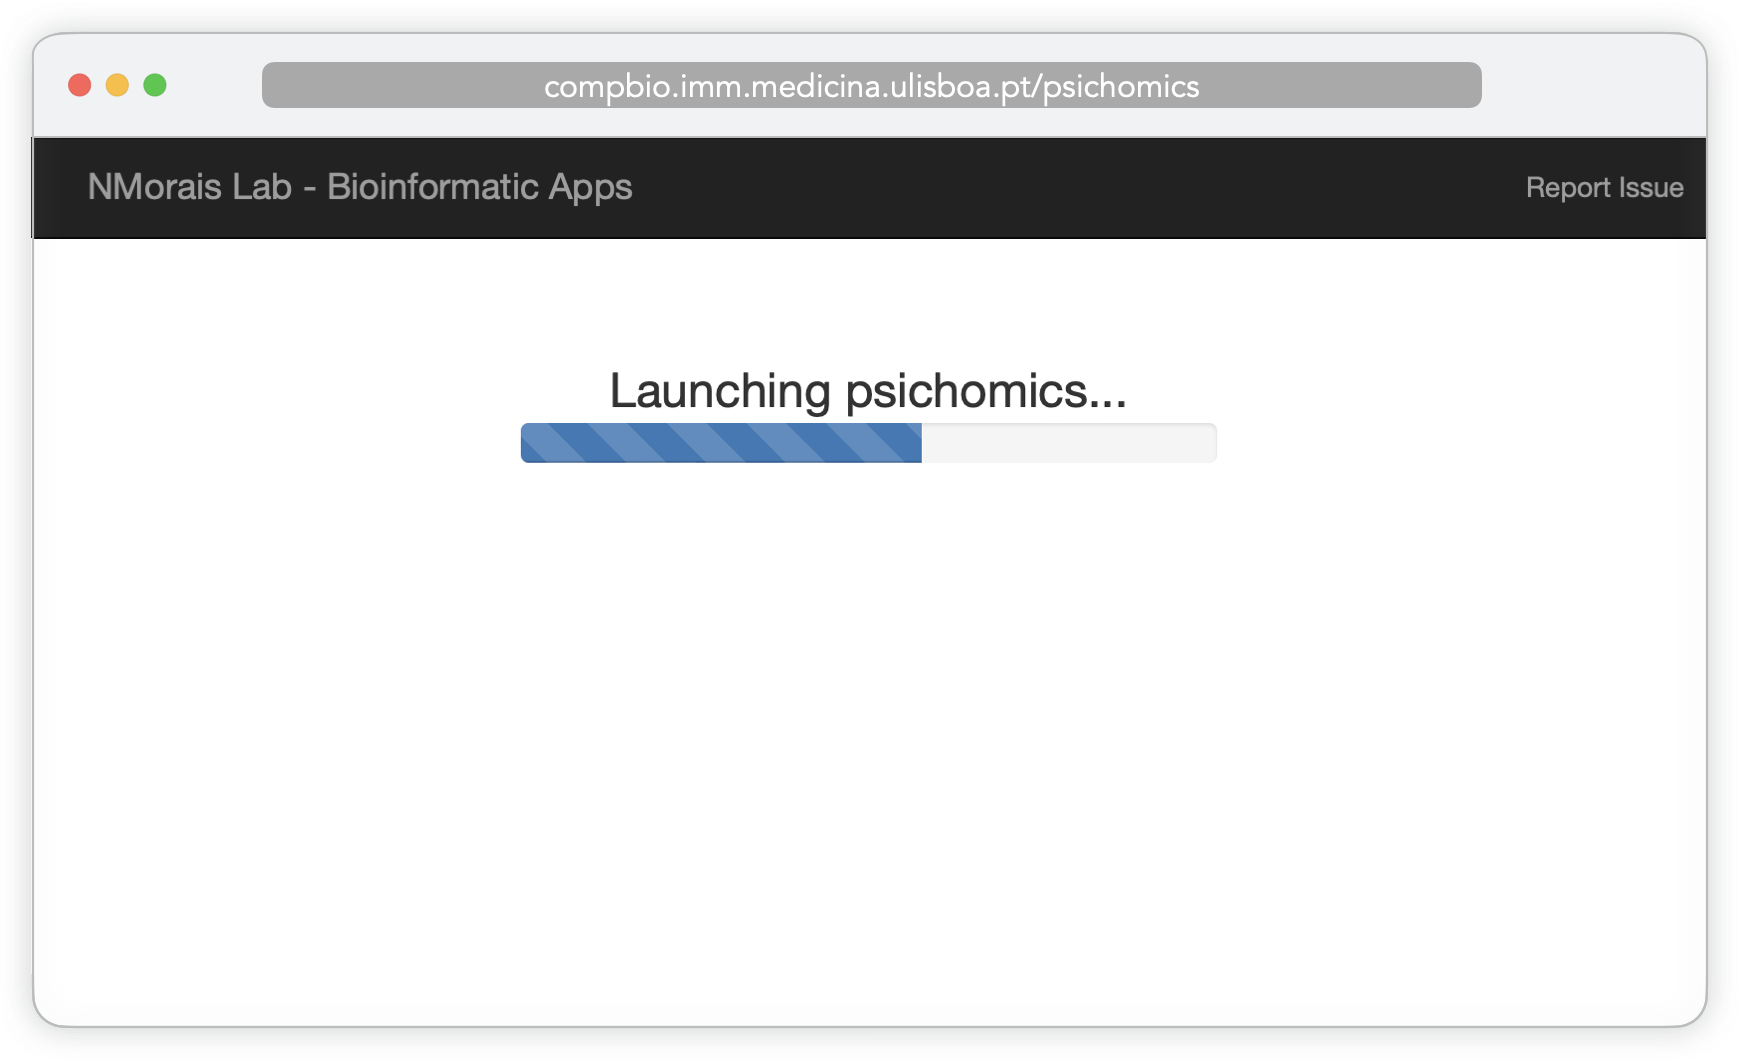
\includegraphics[width=\linewidth]{images/app-server/progress-bar}
  \caption[Screenshot of app loading]{\textbf{Progress bar displayed while psichomics loads} (11 Nov 2021).}
  \label{fig:progress-bar}
  \vspace{-\intextsep}
\end{wrapfigure}

% https://dl.acm.org/doi/pdf/10.1145/1294211.1294231
% https://www.chrisharrison.net/index.php/Research/ProgressBars2
% https://dl.acm.org/doi/pdf/10.1145/2702123.2702139
% https://www.researchgate.net/publication/234791131_The_importance_of_percent-done_progress_indicators_for_computer-human_interfaces
% https://ieeexplore.ieee.org/stamp/stamp.jsp?tp=&arnumber=6263888&tag=1

When ShinyProxy is loading an app, a spinning wheel is shown as a loading indicator. For apps that take more than 10 seconds to load (e.g. psichomics and cTRAP), the user may think the website is not working and close the window before the app is loaded. To avoid that, the spinning wheel was replaced with a progress bar to provide a time estimate for app loading (\autoref{fig:progress-bar}), making wait times more tolerable \cite{myers:1985aa,yablonski:2020ts}.

\bigskip
\bigskip

By default, the progress bar takes 5 seconds to fill (as sample Shiny apps take that much to launch in ShinyProxy), but the time is customisable for specific apps by editing the ShinyProxy configuration file (\texttt{shinyproxy/application.yml}) and adding a \texttt{template-properties.start-up} parameter to a specific app. For instance, psichomics takes 20 seconds to fully load the progress bar (i.e. \texttt{template-properties.start-up: 20s}), whereas cTRAP takes 15 seconds. When the app finishes loading, the progress bar is replaced by the app regardless of the progress displayed to the user. The accuracy of the progress bar does not need to be perfect to serve its purpose \cite{myers:1985aa,yablonski:2020ts}.

To create this progress bar, \verb|shinyproxy/templates/app.html| was edited to remove the spinning wheel and to include an empty progress bar. The progress bar's width is changed from 0\% to 100\% using JavaScript. By default, the CSS width transition applied to the progress bar is \texttt{transition: width 5s ease-in-out;} (animating a change of width that last for 5 seconds in an ease-in animation) where \texttt{5s} is replaced by the \texttt{template-properties.startup-time} parameter if set.

% \subsubsection{Report issue}

% The report issue button creates an email based on the page it is.

\subsubsection{Private web apps}

In the website's landing page (\autoref{fig:homepage}), ShinyProxy lists all apps described in the configuration file by default (\texttt{shinyproxy/application.yml}). This may not be desired when hosting apps with confidential results to be shared with specific collaborators. For this reason, we added the key \texttt{template-properties.listed} that can either be \texttt{false} (default) or \texttt{true}. The file \texttt{shinyproxy/templates/index.html} was edited to show only apps whose \texttt{template-properties.listed} key is set to \texttt{true}. Thus, non-listed web apps are not displayed in the landing page, but are still directly accessible via URL based on their app ID, e.g. \alink{compbio.imm.medicina.ulisboa.pt/app/psichomics}.

However, if the information contained in the web app should not be accessible to strangers at all, apps can also implement a password input form (e.g. \texttt{shiny::passwordInput()}) in the code itself before loading any data and/or information. That password should be securely shared with the intended audience only.

\subsection{Nginx}

Nginx is a reverse proxy, i.e. an intermediary that controls what is shown to the user depending on the URL visited -- akin to those switchboard operators seen in old movies. In CompBio, Nginx fulfills user requests and performs many other functions:

\begin{itemize}
	\item \textbf{Ensure HTTPS traffic is encrypted via SSL certificates} from the IT team at iMM. We simply point to the correct location of those certificates.%As standard practice, the certificates are composed by three parts: the site certificate, intermediate certificates, and the private key.
	\item \textbf{Serve publicly available files} in the \texttt{nginx/public} folder, whose directory structure is accessible at \alink{https://compbio.imm.medicina.ulisboa.pt/public/}.
	\item \textbf{Show a custom error page if ShinyProxy is not responding} (e.g. temporarily down or overloaded). When ShinyProxy is down, Nginx informs end-users to retry refreshing the page and that ShinyProxy is probably down, informing end-users to retry refreshing the page. ShinyProxy can be down for multiple reasons, such as during a restart or due to resource overloading. % custom HTML error page screenshot?
	\item \textbf{Display the website favicons} stored in folder \texttt{nginx/favicon}.
\end{itemize}

\subsection{Background tasks}
\label{sec:background-tasks}

In our app server, we use Celery to run background tasks, alongside Flower to manage Celery jobs via its graphical interface and HTTP API\footnote{More information in \fullref{subsec:background-tasks}.}. We also use the Redis broker to communicate between the two Docker containers.

Currently, cTRAP is the only web app in our server that exploits background tasks. We built a Docker image based on the official cTRAP Docker image (\dockerlink{nunoagostinho/ctrap}) with the Celery app installed on top.

% --max-memory-per-child
% --time-limit and --soft-time-limit
% --autoscale=10,3
Celery was configured to use 3 to 10 processes based on demand, as well as CPU and memory usage via an independent plugin (\alink{github.com/jcushman/celery-resource-autoscaler}). For instance, each process in Celery can use up to 10GiB of RAM and run up to 12 hours, thus avoiding rogue tasks.

To run other programs in Celery, we need to create a custom Dockerfile containing those programs (e.g. based on their Docker images) with Python and Celery installed. The Nginx configuration needs to include the new Celery service (\shortref{lst:celery-worker}).

\begin{lstlisting}[caption=Configuration of the Celery service for cTRAP in \texttt{docker-compose.yml}.,language=XML,label={lst:celery-worker}]{celery-worker}
  celery-ctrap:
    container_name: celery-ctrap
    build: ./celery
    command: celery -A tasks worker -c5 -l info -E -n ctrap
    volumes:
      - ./celery:/celery:ro
      - ../apps/cTRAP/sessions:/data
    depends_on:
      - redis
\end{lstlisting}

\subsection{Resource monitoring}

Prometheus monitors the server resources and the collected data can be visualised using Grafana (\shortref{fig:grafana}). The tracked resources include Celery job usage, ShinyProxy metrics (app usage time, app failures, users per app, etc.), Nginx status and Linux system resources (e.g. RAM usage, available disk space and CPU stress).

\begin{figure}[!h]
	\centering
	\begin{subfigure}[h]{0.45\textwidth} 
		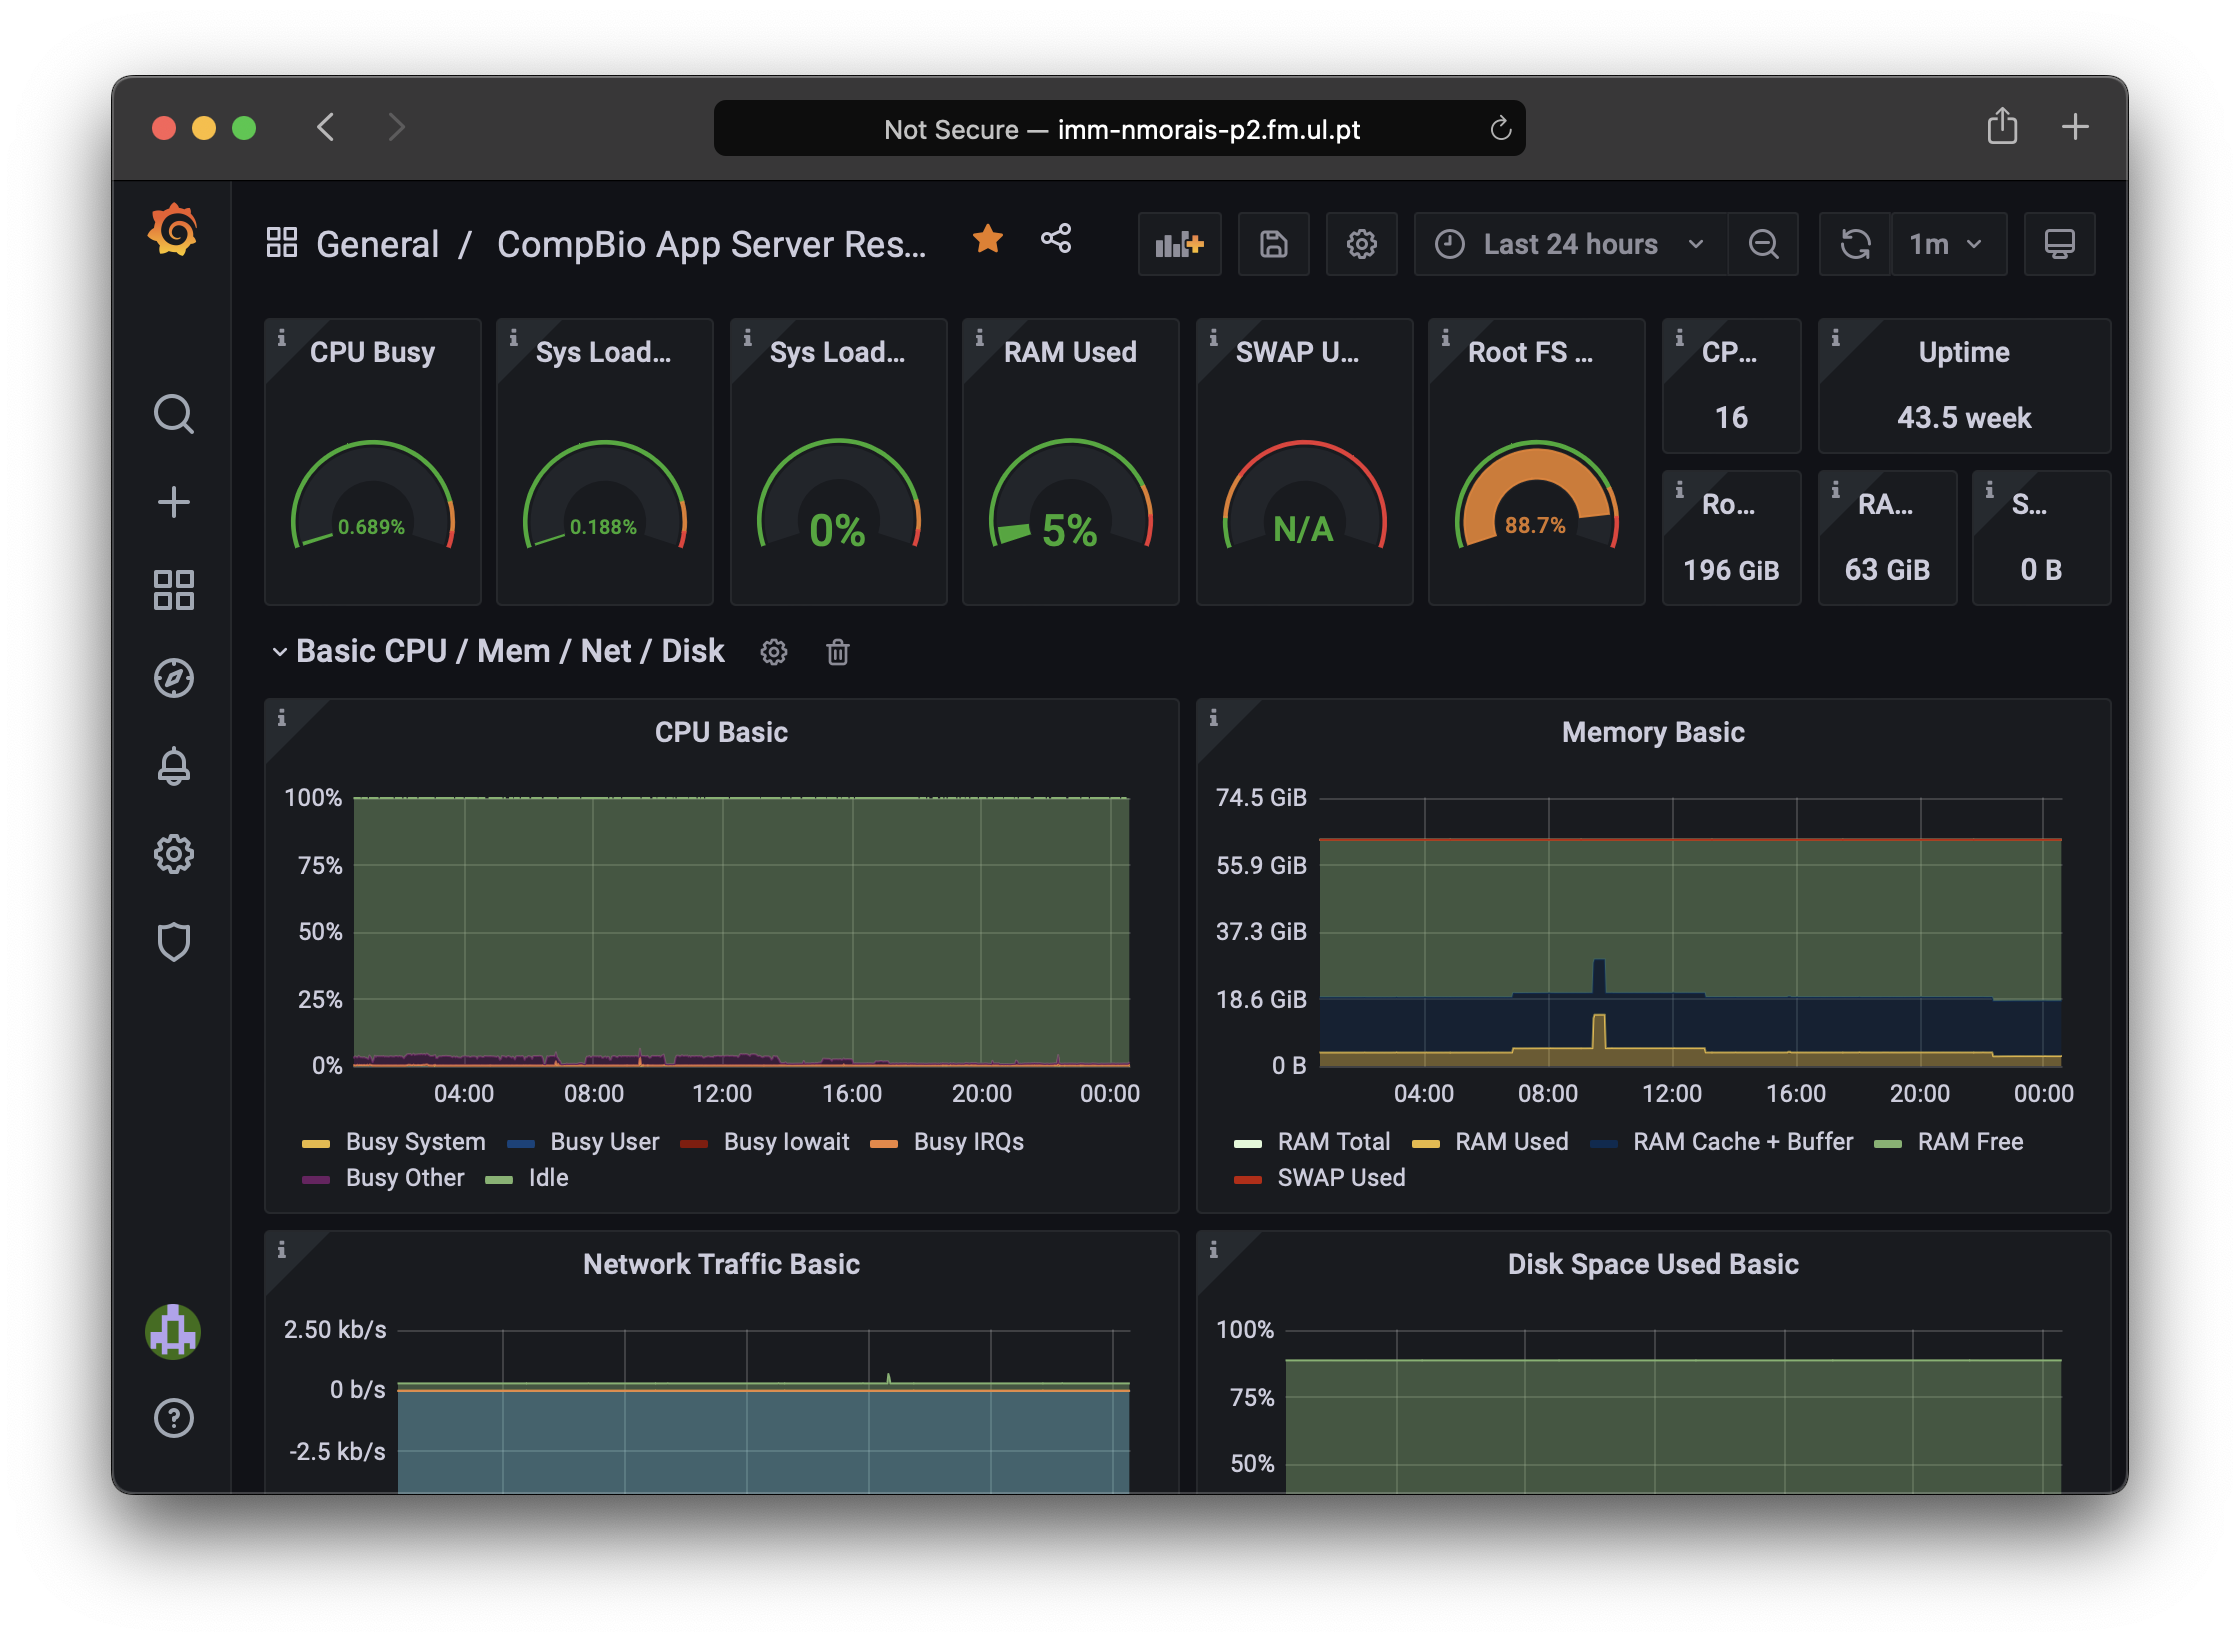
\includegraphics[width=\textwidth]{images/app-server/grafana-system}
		\caption{Linux system metrics.}
	\end{subfigure}
	\begin{subfigure}[h]{0.45\textwidth}
		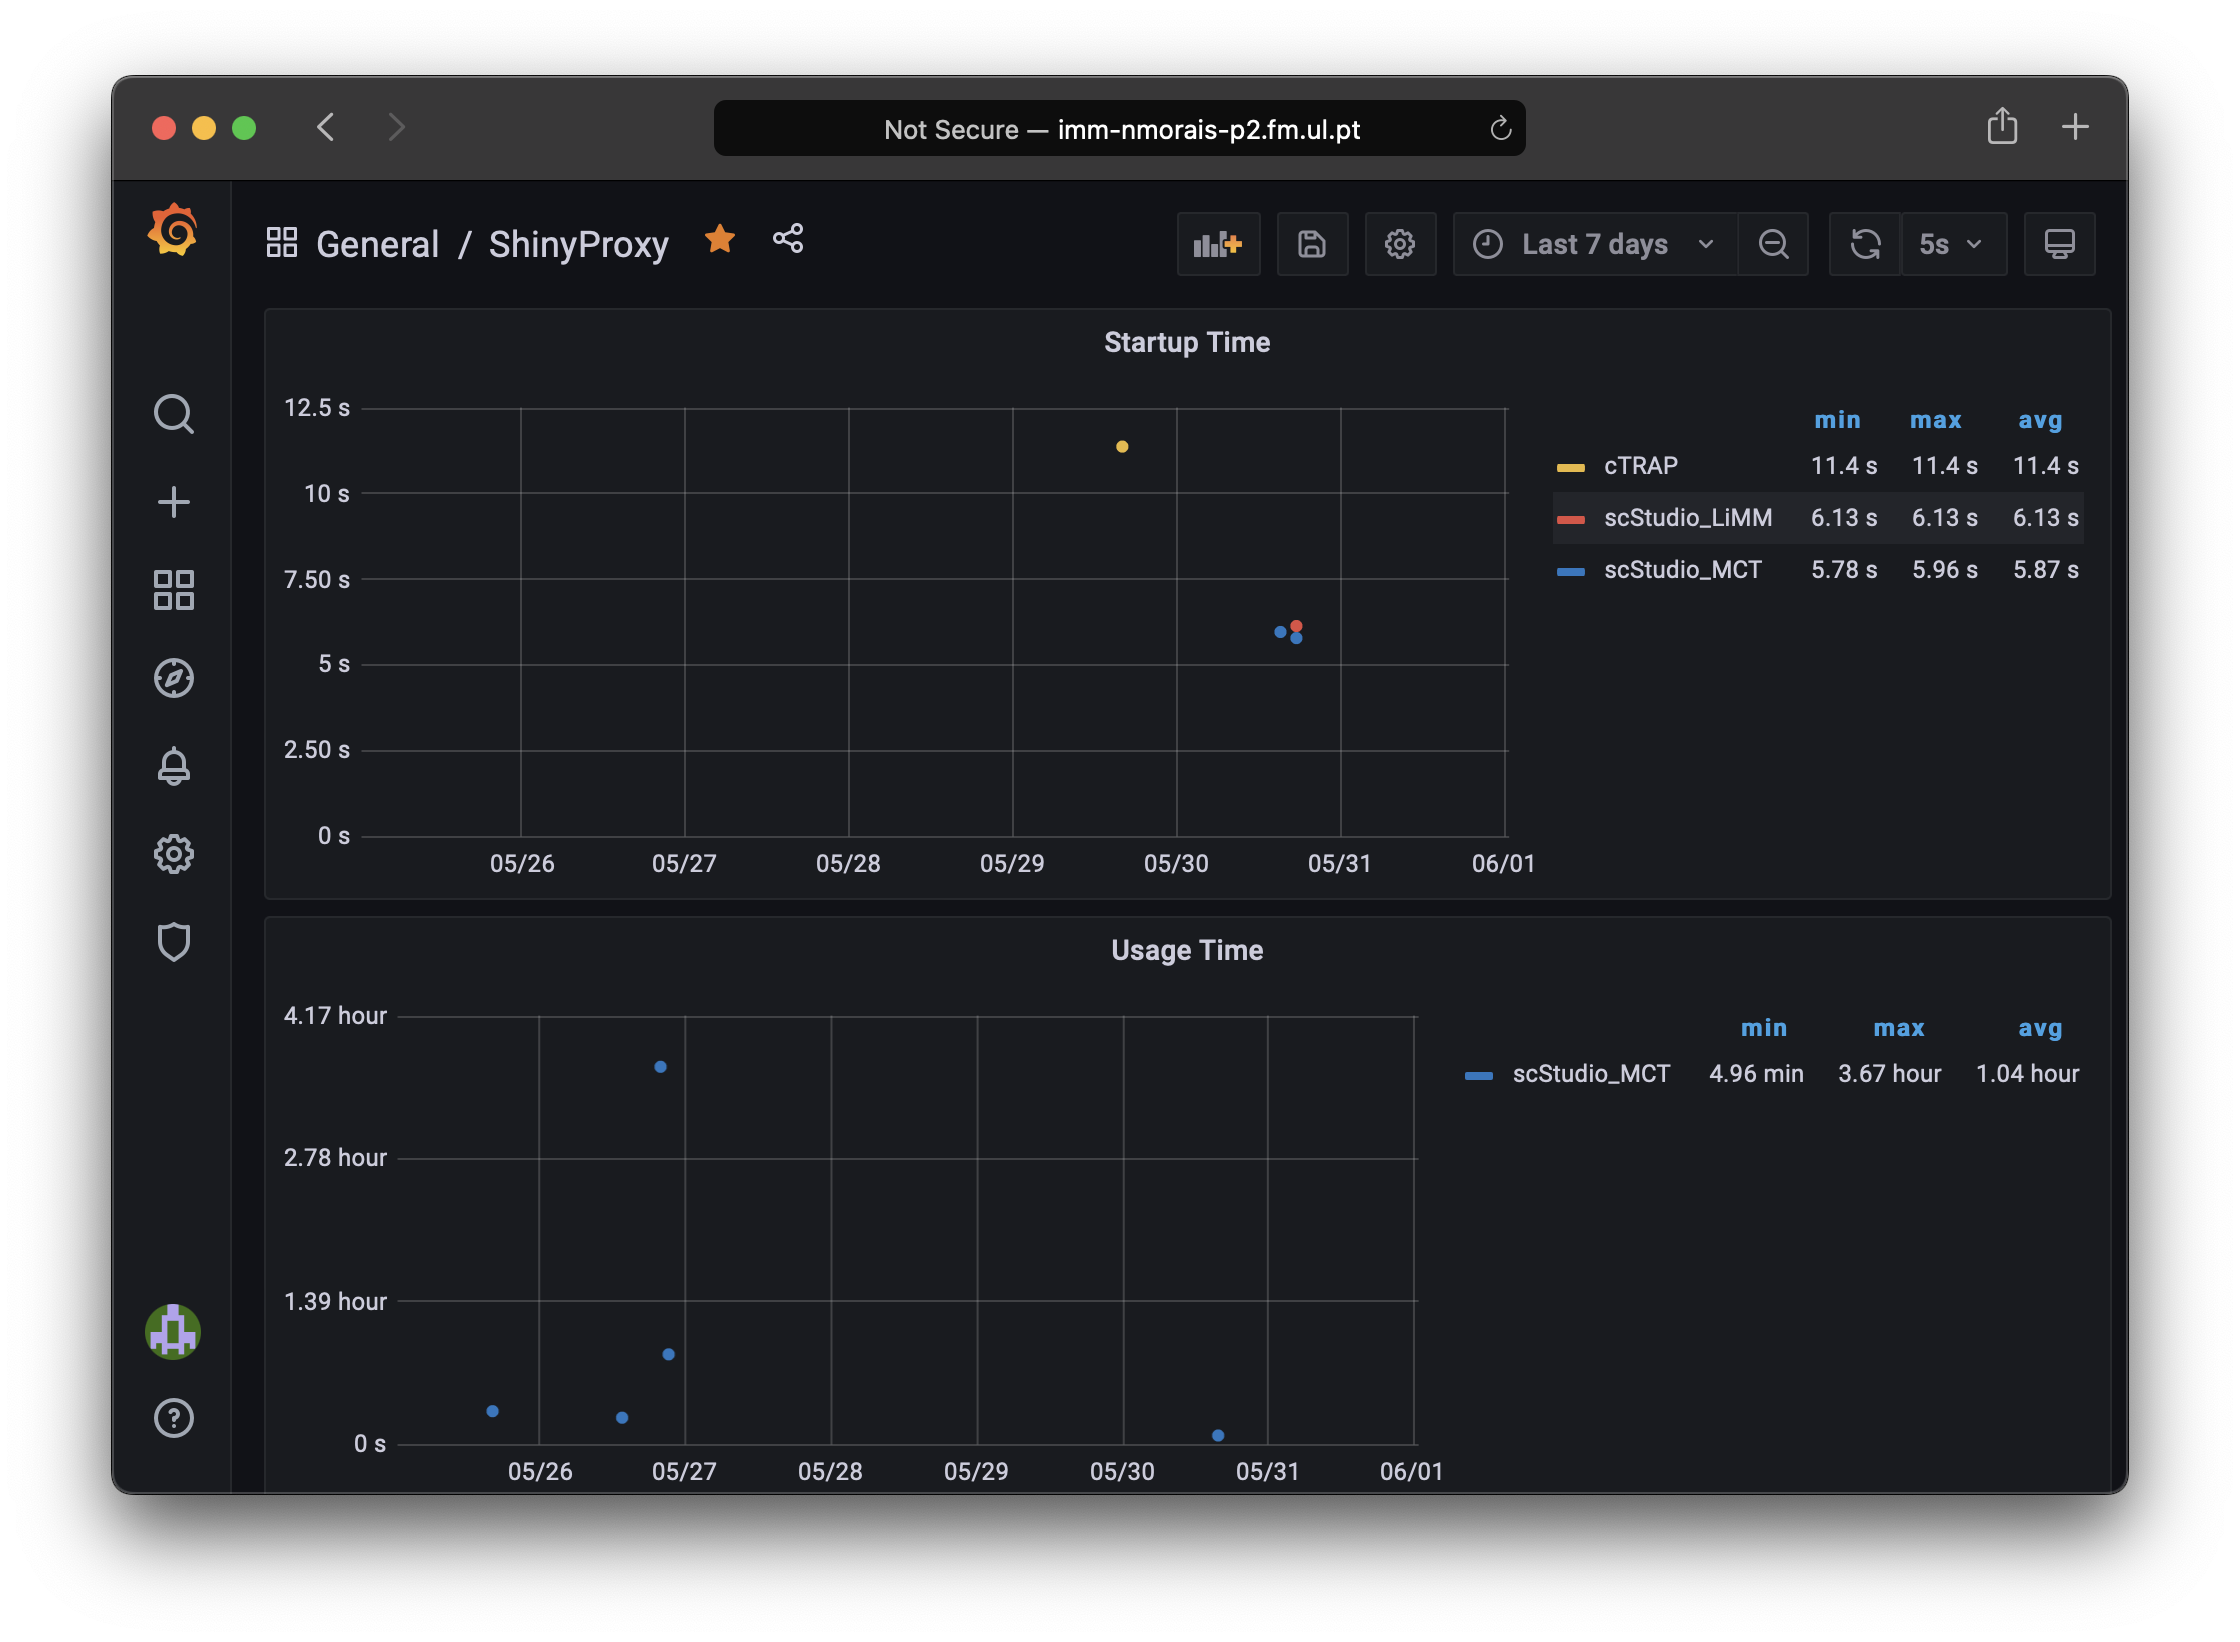
\includegraphics[width=\textwidth]{images/app-server/grafana-shinyproxy}
		\caption{ShinyProxy metrics.}
	\end{subfigure}
	\begin{subfigure}[h]{0.45\textwidth}
		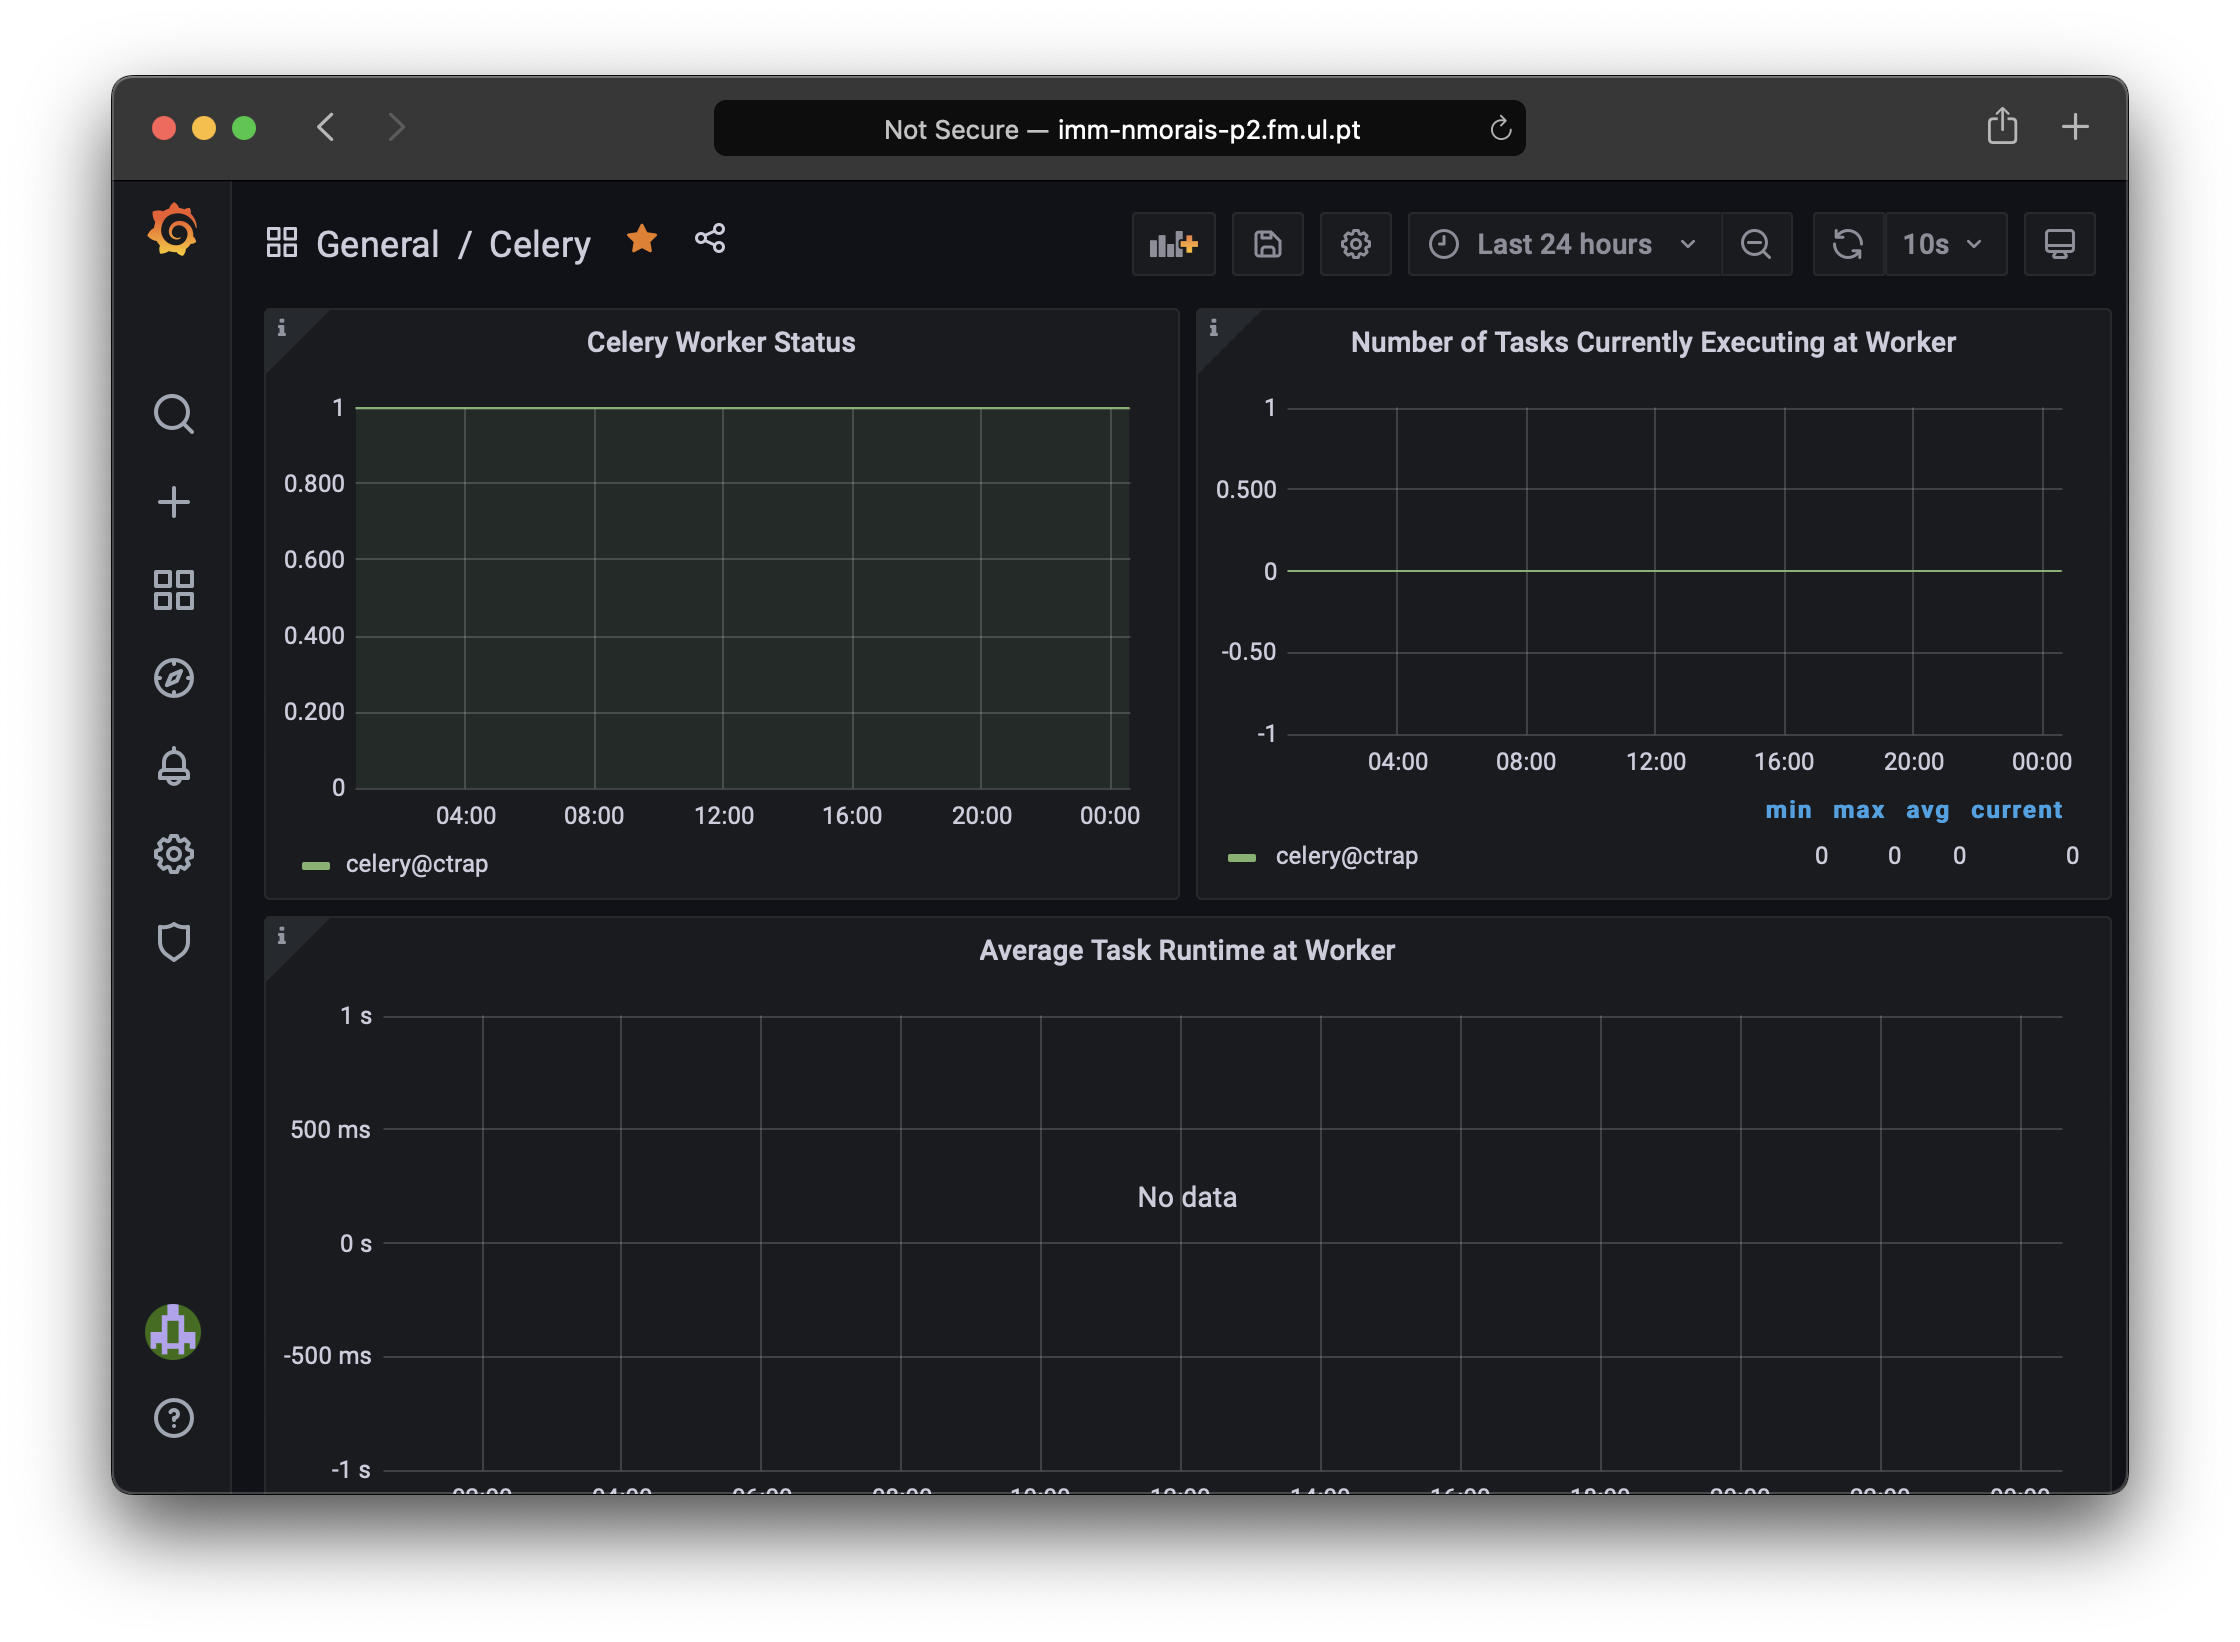
\includegraphics[width=\textwidth]{images/app-server/grafana-celery}
		\caption{Celery metrics.}
	\end{subfigure}
	\begin{subfigure}[h]{0.45\textwidth}
		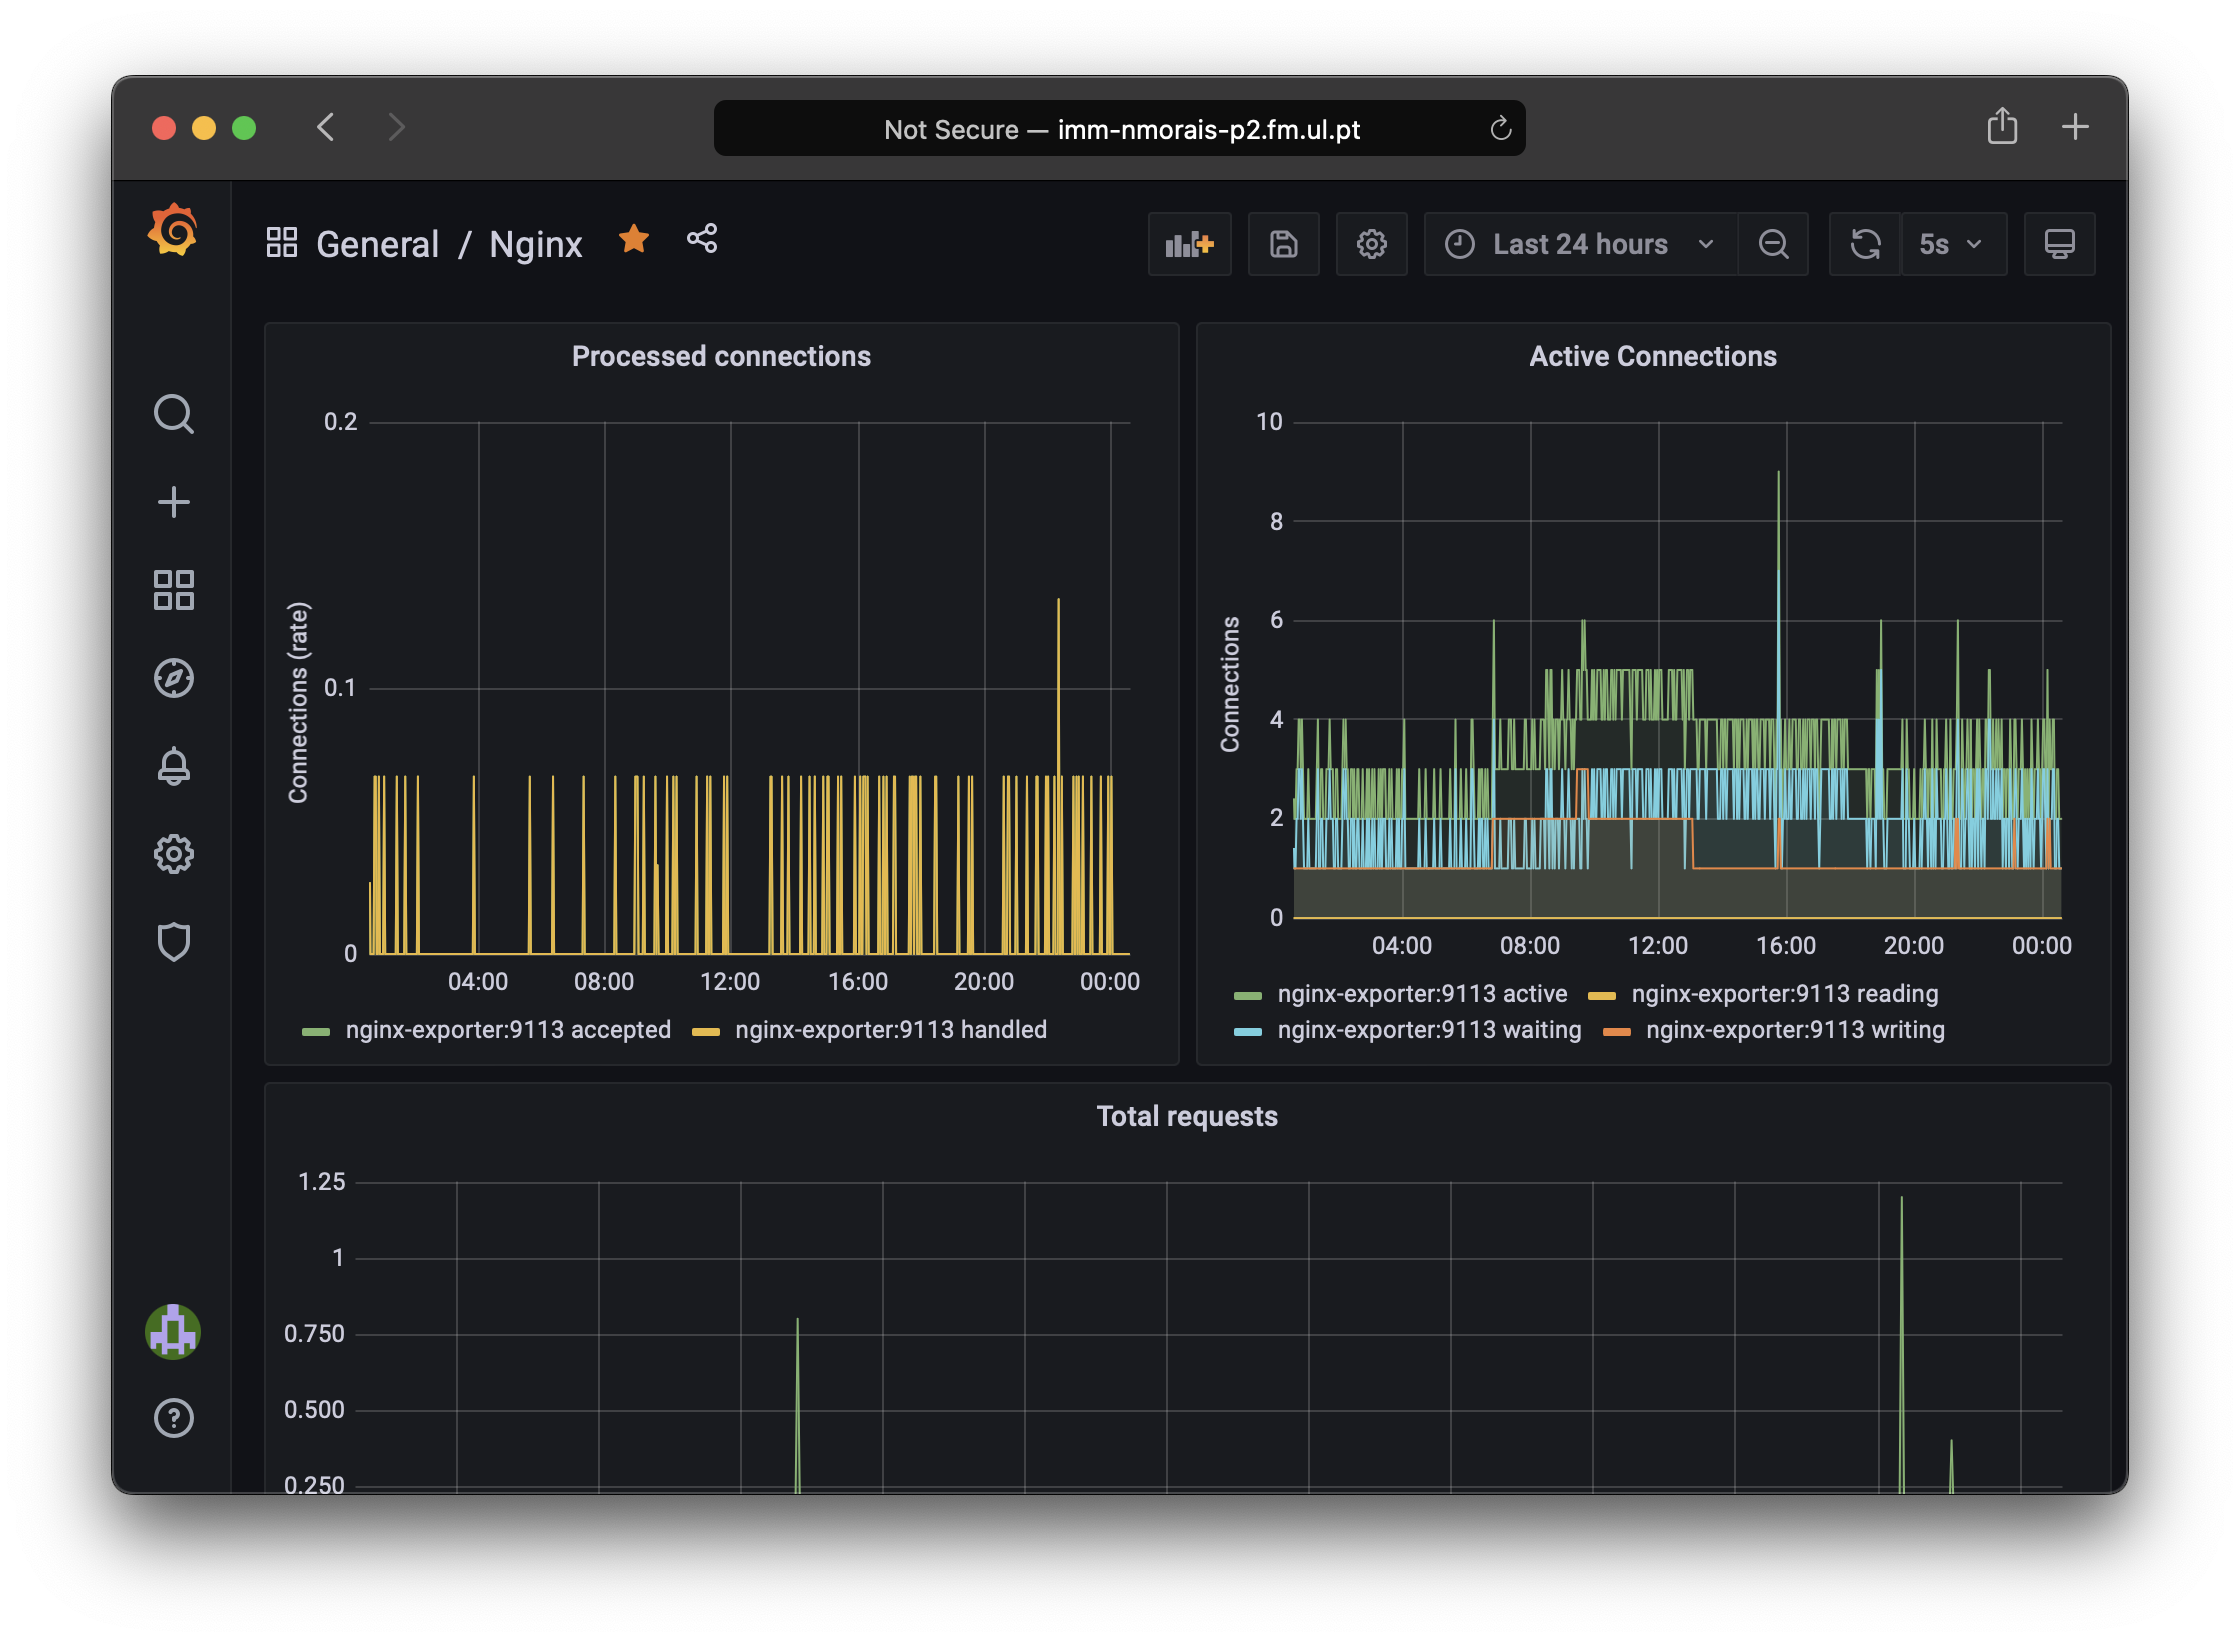
\includegraphics[width=\textwidth]{images/app-server/grafana-nginx}
		\caption{Nginx metrics.}
	\end{subfigure}
	\caption[Grafana dashboards]{\textbf{Grafana dashboards} showing tracked metrics (1 Jun 2021).}
\label{fig:grafana}
\end{figure}

\begin{wrapfigure}{r}{.4\textwidth}
  \vspace{-4\intextsep}
  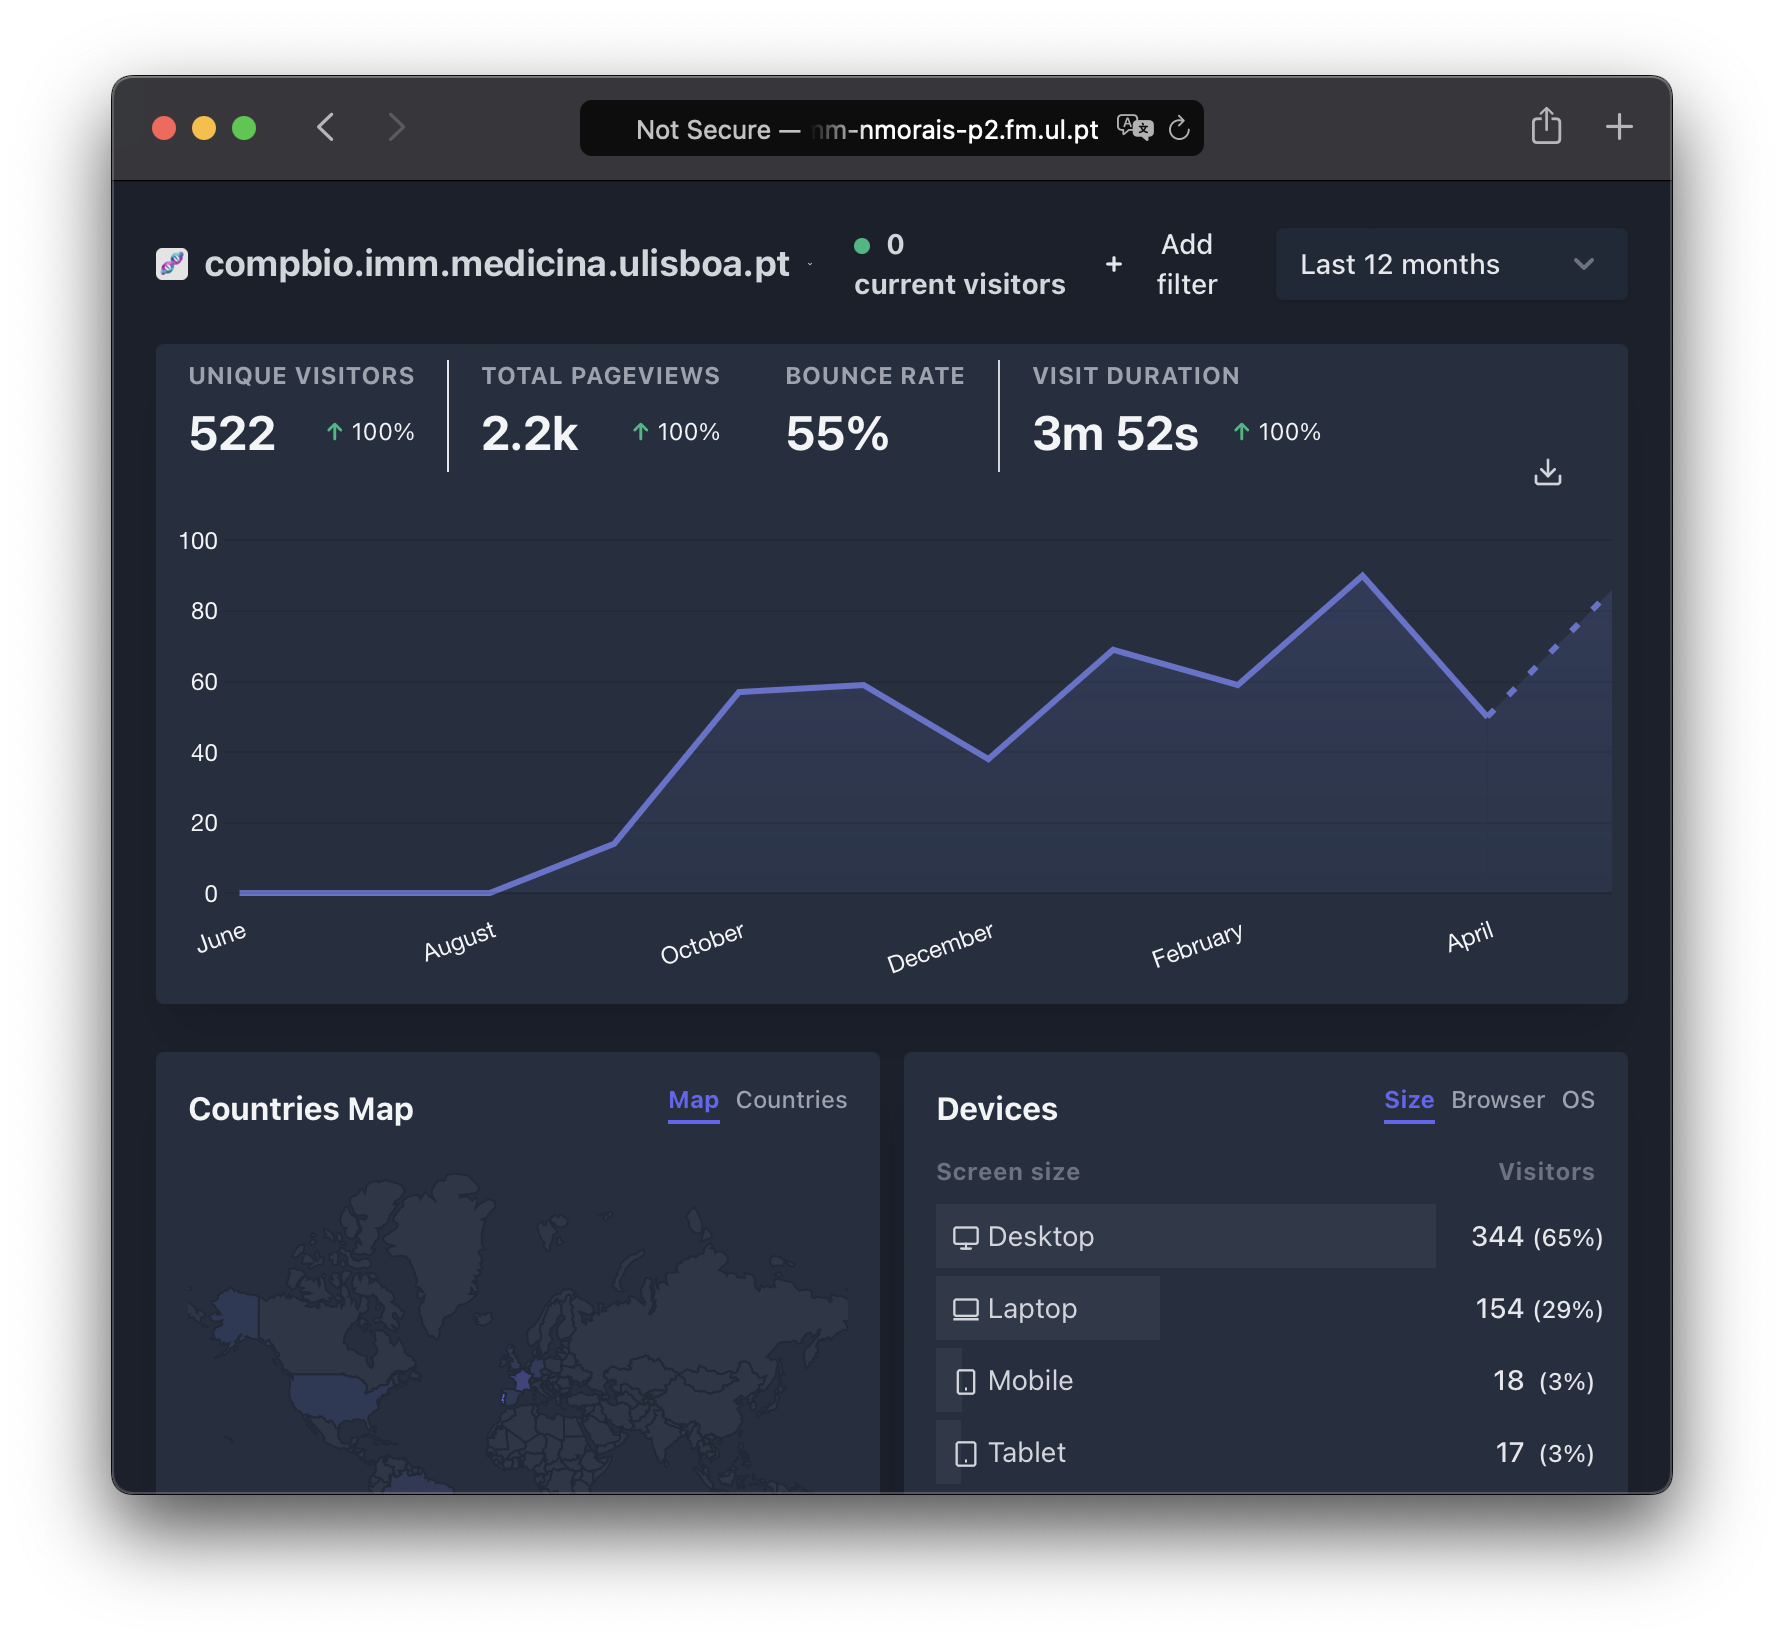
\includegraphics[width=\linewidth]{images/app-server/plausible}
  \caption[Plausible dashboard]{\textbf{Plausible dashboard} showing CompBio website analytics for the last year (as of 31 May 2021).}
  \label{fig:plausible}
  \vspace{-1\intextsep}
\end{wrapfigure}

\subsection{Website analytics}

Plausible is an open-source, privacy-focused web analytics tool that collects traffic metrics for multiple websites and provides them via an interactive dashboard (\shortref{fig:plausible}). CompBio runs the self-hosted version of Plausible. All of Plausible metrics (e.g., visitor numbers, total page views and session duration) are anonymously aggregated without cookies, thus avoiding individual tracing of users.

Plausible uses the database management systems ClickHouse and PostgreSQL to store tracking data. PostreSQL can also be used in the future as the SQL database of the server if desired, although currently no web apps in the server use this database.

Using the self-hosted version of Plausible guarantees that the tracking of user data is performed locally in the server. Plausible also protects user privacy by making their data hard to individually trace and by complying with current privacy laws. %(GDPR, CCPA and PECR).

\subsection{Server maintenance}

% TODO: Run Docker images as rootless

CompBio is a web server that hosts Shiny applications and is publicly accessible by everyone online. This makes our server a target for potential security attacks. In order to mitigate such vulnerabilities, it is crucial to update its components, including Docker, Docker Compose, Nginx and ShinyProxy. As updates may contain breaking changes that hamper website functionality, it is recommended to read change logs related to new software versions to pinpoint potential issues before updating.

% https://www.sciencedirect.com/science/article/pii/S2352484721007289#b71
% https://doi.org/10.1145/3038923
% https://www.tandfonline.com/doi/full/10.1080/19393555.2020.1853855?casa_token=EpT3lJflBXAAAAAA%3AaS5ePDNIcAPfL6MsMoKrI0s4sDtjyGNvGICZiz2Ywvnf7E2vtokORb073GUi9eilZiUCFOAqhIY

Updates to Docker and Docker Compose need to be performed by an administrator using Linux's \texttt{apt-get} command\footnote{sudo apt-get update \&\& sudo apt-get upgrade}. On the other hand, Docker images of the server (including Nginx and ShinyProxy) require a user in the \texttt{docker} group to edit the versions of the Docker images used in \texttt{docker-compose.yml} and restart the Docker Compose project\footnote{While inside the project folder: \texttt{docker compose down \&\& docker compose up -d --build}}. The advantage of using Docker Compose is that if something goes wrong with the updated Docker images, we simply need to revert \texttt{docker-compose.yml} to a previous working state and restart all services.

\section{Conclusion}

% what is your main finding (ANSWER)
% how are your findings with respect to the literature (POSITIONING)
% - RESULT: the actual results
% - CONTEXT: literature search
% - LINK: between my findings and what is known
% - INTERPRETATION: where you pinpoint, suggest, propose...
% what is your main contribution (CONTRIBUTION)
% what are the limitations (LIMITATIONS)
% what are the next steps (ENDING/FUTURE WORK)

The CompBio app server was developed to host web apps from NMorais Lab using ShinyProxy and Docker Compose, allowing to easily add new or update existing Shiny apps containerised via Docker. It also contains multiple components to run background cTRAP tasks, track app usage and monitor computing resources.

CompBio currently runs in a virtual machine in Lobo, iMM computing cluster. The hardware is taken care by the iMM IT team and they also support us with issues regarding SSL certificates, WebSocket connections and resource allocation. Moreover, I expect the server components to be easy to maintain and update. Components can be manually updated by simply editing the intended version in \texttt{docker-compose.yml} and restarting all the services. In case of issues, it is easy to rollback to a stable, working version of the app server based on previously used Docker images. Testing new changes to the server can be performed using the staging mode, allowing to mirror the app server and test changes locally before pushing them live to the app server.

The project also makes uses of Nginx as a reverse proxy. An issue with using Nginx is that it is especially verbose compared to more recent reverse proxies. Although I would have liked to replace Nginx with a simpler reverse proxy -- such as Caddy (\alink{caddyserver.com}) --, Nginx is more popular and widely used, thus making it easier to find documentation and to search for issues.

In the future, we can adapt available computing resources of our virtual machine as needed. In case we prefer to port the app server to a new machine, as the project was built on Docker Compose, relocating the app server is as easy as moving the project data to the new machine, installing Docker and Docker Compose, downloading required Docker images and starting the app server as previously indicated.

By publicly hosting the project code in GitHub, we hope to demonstrate the flexibility of setting up Docker Compose to other labs and entities, promoting an easily portable, reproducible and documented configuration of a Shiny web app server that can facilitate sharing public apps among the scientific community and beyond.
